% 	This template is  MIT licensed.

% 	Basic file to demonstrate the usage of this LaTeX template.
% 	You can build your own paper/thesis on top of this file.
% 	Simply adjust the document class and all metadata and start working.
%
\documentclass[
	language=english, % set to english or german
	type=master, % set to bachelor, master or seminar
]{isthesis}

\usepackage[utf8]{vntex}
% \usepackage[vietnamese]{babel}

% custom package
\usepackage{eurosym}
\usepackage{makecell}
\usepackage{hyperref}
\usepackage[utf8]{inputenc}
\usepackage{tabto} 
\usepackage{longtable}
% \usepackage{multirow}
% \usepackage{floatrow}

% Graphics rendering using TikZ
% See: https://en.wikibooks.org/wiki/LaTeX/PGF/TikZ
\usepackage{tikz}
\usepackage{xcolor}
\definecolor{light-gray}{gray}{0.95}
\newcommand{\code}[1]{\colorbox{light-gray}{\texttt{#1}}}
% Include required TikZ libraries here, some exemplary libraries are pre-included
\usetikzlibrary{calc}
\usetikzlibrary{matrix}
\usetikzlibrary{positioning}
\usetikzlibrary{shapes.geometric}

%Add your library here
\addbibresource{library.bib}

% Import acronyms
% \newacronym[longplural={<long plural>}, shortplural={<short plural>}]{<label>}{<short>}{<long>}
% 	label = is the unique identifier and sort key for the acronym, can be the same as <short>
%	short = is the abbreviation or acronym
%	short plural (optional) = is the plural of the abbreviation or acronym
%	long = is the long form of the acronym, this will appear in the list of abbreviations
%	long plural (optional) = is the long plural form of the abbreviation or acronym

\newacronym[shortplural={KMUen}, longplural={Kleine und Mittlere Unternehmen}]{kmu}{KMU}{Kleines und Mittleres Unternehmen}
\newacronym{CD}{CD}{Corporate Design}
\newacronym{SQL}{SQL}{Structured Query Language}
\newacronym{FAU}{FAU}{Khoa Toán cơ tin}
\newacronym{BPM}{BPM}{Business Process Management}
\newacronym{npm}{NPM}{Node Package Manager}
\newacronym{diss}{DISS}{Digital Industrial Service System}

% Import symbols
% Syntax: <Symbol> <Label> <Name>
% The symbols are sorted by their labels
\addsymboltolist{$\Pi$}{Pi}{Projection}
\addsymboltolist{$\Join$}{Join}{Natural Join}
\addsymboltolist{$\sigma$}{Selection}{Selection}


% Import custom commands
% If you want to define custom commands, please do so here

% Import custom code block
% define listing code
\definecolor{codegreen}{rgb}{0,0.6,0}
\definecolor{codegray}{rgb}{0.5,0.5,0.5}
\definecolor{codepurple}{rgb}{0.58,0,0.82}
\definecolor{backcolour}{rgb}{0.95,0.95,0.92}

\lstdefinestyle{code}{
    backgroundcolor=\color{backcolour},   
    commentstyle=\color{codegreen},
    keywordstyle=\color{magenta},
    numberstyle=\tiny\color{codegray},
    stringstyle=\color{codepurple},
    basicstyle=\ttfamily\footnotesize,
    breakatwhitespace=false,         
    breaklines=true,                 
    captionpos=b,                    
    keepspaces=true,                 
    numbers=left,
    firstnumber=1,
    stepnumber=1,                    
    numbersep=5pt,                  
    showspaces=false,                
    showstringspaces=false,
    showtabs=false,                  
    tabsize=2,
    framesep=10pt,
    xleftmargin=10pt,
    xrightmargin=10pt,
    framexleftmargin=16pt,
    framextopmargin=2pt,
    framexbottommargin=2pt, 
    frame=tb, framerule=0pt,
}

\lstdefinestyle{algo}{
    backgroundcolor=\color{backcolour},   
    commentstyle=\color{codegreen},
    keywordstyle=\color{magenta},
    numberstyle=\tiny\color{codegray},
    stringstyle=\color{codepurple},
    basicstyle=\ttfamily\footnotesize\small\linespread{0.8},
    breakatwhitespace=false,         
    breaklines=true,                 
    captionpos=b,                    
    keepspaces=true,                 
    numbers=none,
    firstnumber=1,
    stepnumber=1,                    
    numbersep=5pt,                  
    showspaces=false,                
    showstringspaces=false,
    showtabs=false,                  
    tabsize=2,
    framesep=10pt,
    xleftmargin=10pt,
    xrightmargin=10pt,
    framexleftmargin=16pt,
    framextopmargin=2pt,
    framexbottommargin=2pt, 
    frame=tb, framerule=0pt,
    mathescape=true
}

\lstset{style=code}

% Document meta information
\isthesis{
    title={TIỂU LUẬN},
    sub-title={Toán rời rạc và thuật toán\\ Phương pháp tìm kiếm lân cận rộng thích ứng \\ cho bài toán lấy và giao hàng với ràng buộc thời gian},
    author-name={Nguyễn Mạnh Linh, Nguyễn Thị Đông, Triệu Hồng Thuý}, 
    % Separate multiple authors with commas
    % author-email={linhnguyen.code@gmail.com},
    % author-matriculation={MATRICULATION NUMBER},
    % author-phone={+49 XXXXXXXXX}, % Use international numbers format
    % author-address={STREET},
    % author-zip={ZIP},
    % author-city={CITY},
    principal-supervisor={PGS.TS. Nguyễn Thị Hồng Minh}, % This must be a professor
    % associate-supervisor={SUPERVISOR}, % This is your main supervisor, i.e., a post doc or doctoral student
    tutor-supervisor={}, % If required, define an additional supervisor resp. tutor here
    group-institute={Đại học Khoa học Tự nhiên},
    % group={Image Data Exploration and Analysis (IDEA) Lab},
    % studies={M.Sc. International Information Systems}, %your field of studies, i.e. Wirtschaftsinformatik or International Information Systems
    %
    %associate-group={}, % When the thesis is done in cooperation with another chair, add it here
    %associate-group-institute={}, % add cooperating institute or university here
    seminar={SEMINAR}, % The title of your seminar
    submission-date={2023-02-01}, % The date you handed in your document: Format yyyy-mm-dd
    primary-logo={assets/hus.png}, % Uses the FAU logo by default
    %primary-logo-height={}, % Uses 16mm as default height
    %secondary-logo={}, % Logo of the secondary institution (cooperating chair/university), USES Faculty logo by default
    %secondary-logo-height={} % Uses 16mm as default height
}


\begin{document}
    % Title page
    \newcounter{savepage}
    \maketitle

	% Quote
    % You can put an optional quote page in front of your content
    %   \quotepage[author={Arthur C. Clarke}]{
    %   	        Any sufficiently advanced technology is indistinguishable from magic.
    %   }
    
    % Table of contents
    \tableofcontents

    \begin{abstract}
    Ngoài việc lập trình thì vận hành và giám sát là khâu quan trọng trong vòng đời của một sản phẩn công nghệ (phần mềm). Vận hành một sản phẩm không hề dễ dàng hơn việc tạo ra nó. Khi một phần mềm được triển khai thực tế, lập trình viên cũng như người quản trị hệ thống luôn cần nắm rõ \textit{sức khoẻ} của sản phẩm ví dụ như phần mềm đang tiêu tốn bao nhiêu tài nguyên của máy tính, phần mềm xử lý yêu cầu nhanh hay chậm, hay có bao nhiêu lỗi xảy ra trong khung giờ... Những thông số hay độ đo này là thước đo để biết được sản phẩm có đủ tốt hoặc quan trọng hơn là cảnh báo sớm cho người làm phần mềm về những nguy cơ có thể xảy ra. Bài báo cáo này giới thiệu một loạt các kĩ thuật, độ đo, cách kết hợp những công cụ và việc vận dụng khéo léo giữa bản thân phần mềm (ghi log) và các công cụ đó. Trực quan hoá dữ liệu được sử dụng một cách triệt để nhằm tạo một cái nhìn từ tổng quan đến chi tiết giúp cho người vận hành hệ thống cũng như lập trình viên luôn giữ được phần mềm của mình trong tầm kiểm soát.
\end{abstract} 

    % \begin{abstract}
	%     % Add your abstract here:
        
	% 	% \lipsum[1]
	% \end{abstract}

    % List of figures (if you have figures)
    % \listoffigures

    % List of tables (if you have tables)
    % \listoftables
    
    % List of listings (if you have listings)
	% \lstlistoflistings

    % List of abbreviations (if you use acronyms)
    %\listofabbreviations

    % List of symbols (if you use symbols)
    %\listofsymbols
	
	% Abstract
	%
	% Comment out this part, if you don't require an abstract

	
	% storing the last pagenumber
    \setcounter{savepage}{\value{page}}
    
    
    % Content
    \begin{content}
        % Add your content files:
        \chapter{Giới thiệu}
\begin{figure}[H] % places figure environment here   
  \centering % Centers Graphic
  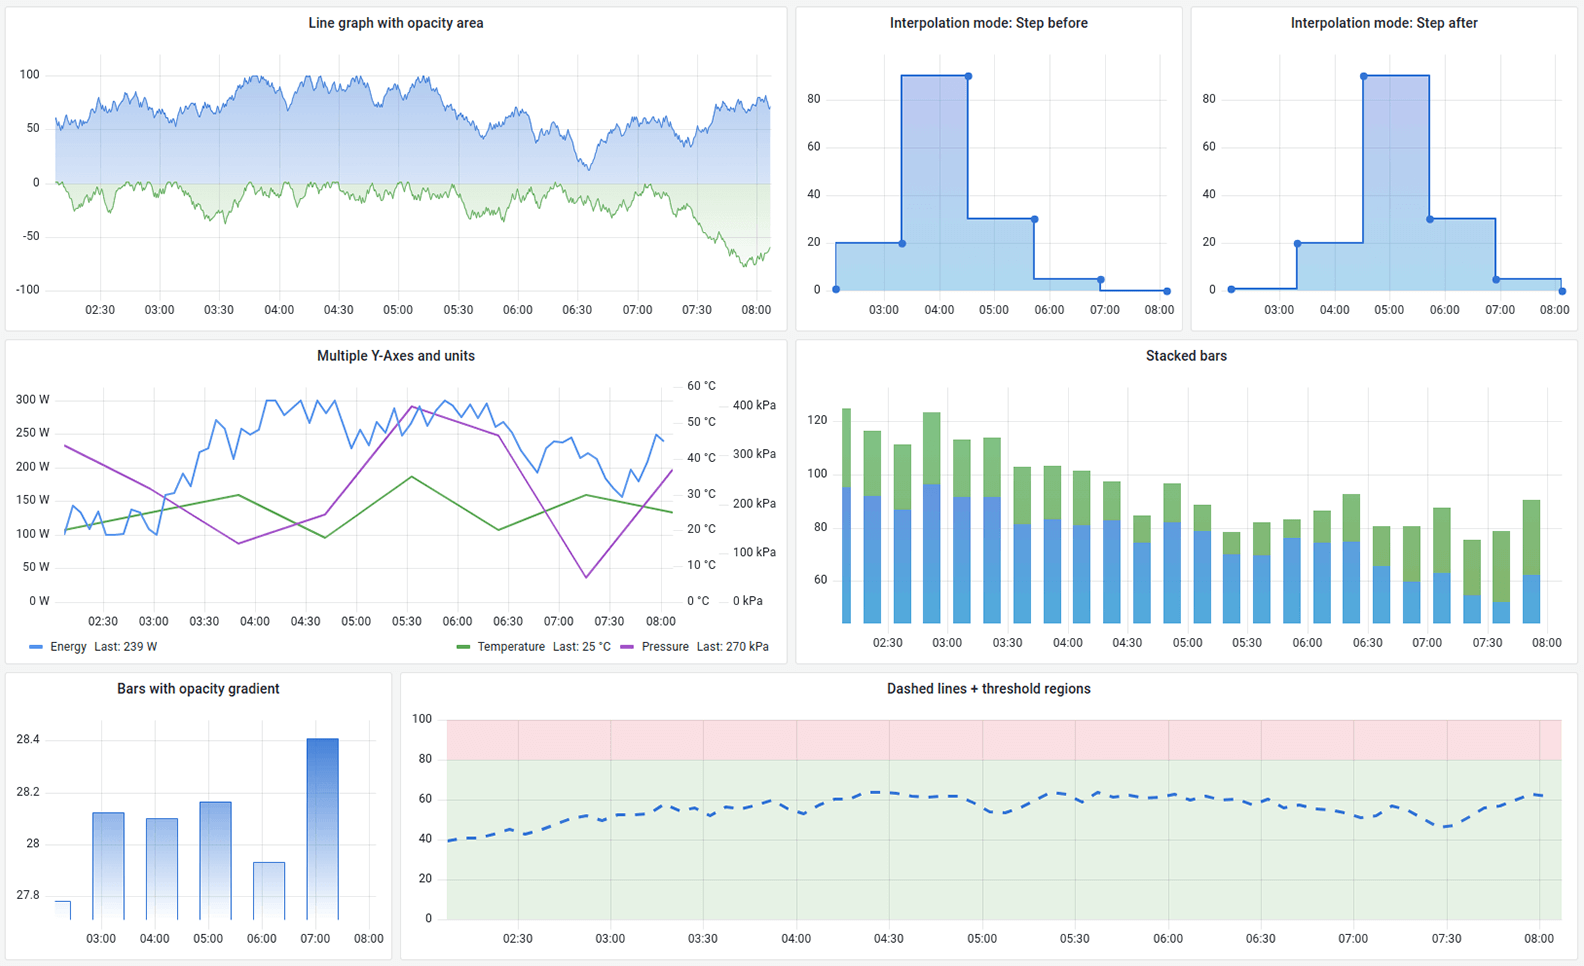
\includegraphics[width=0.8\textwidth]{figures/time_series_light_theme_sized.png} 
  \caption{Biểu đồ dữ liệu hướng thời gian} % Creates caption underneath graph
  \label{fig:fig_01}
\end{figure}

        \chapter{Phương pháp giải}
Tìm kiếm lân cận heuristics thường dựa trên các di chuyển lân cận thay đổi nhỏ so với lời giải hiện tại như là chuyển yêu cầu từ tuyến đường này sang tuyến đường khác hoặc là tráo đổi 2 yêu cầu, như trong bài của Nanry \& Barnes (2000) và Li \& Lim (2001). Những kiểu tìm kiếm lân cận này có thể kiểm tra một lượng lớn phương án trong thời gian ngắn, nhưng phương án được cập nhật rất nhỏ qua mỗi vòng lặp. Đó là điều khiến tác giả tin rằng các phương pháp này có thể gặp khó trong việc di chuyển từ vùng triển vọng này của phương án tới vùng khác khi phải đối mặt với các ràng buộc chặt ngay cả khi áp dụng metaheuristics.

Một trong những cách để giải quyết vấn đề này là cho phép tìm kiếm đi qua các phương án chấp nhận được bằng cách nới lỏng các ràng buộc (ví dụ trong Cordeau, Laporte \& Mercier (2001)). Tác giả chọn một cách tiếp cận khác, thay vì sử dụng bước đi chuyển nhỏ, tác giả sử dụng các bước di chuyển rất lớn mà có thể sắp xếp 30\% đến 40\% tất cả các yêu cầu trong một bước lắp. Sự đánh đổi của việc này là thời gian tính toán cần thiết và việc đánh giá các bước di chuyển trở nên lớn hơn khi so sánh với việc di chuyển các bước nhỏ. Số phương án được đánh giá bởi heuristic tiềm năng trên một đơn vị thời gian chỉ là một phần nhỏ của các phương án được đánh giá trên một heuristic chuẩn. Tuy nhiên, thuật toán cho hiệu năng rất tối trong các bài tests được trình bày trong \$4.

Heuristic tiềm năng dựa trên \textit{large neighbourhood search (LNS)}, được giới thiệu bởi Shaw (1997). LNS heuristic đã được áp dụng vào VRPTW với các kết quả tốt (Shaw 1997, 1998; Bent \& Van Hentenryck 2004). LNS heuristic tương tự với \textit{ruin and recreate} heuristic được trình bày bởi Schrimpf et al. (2000).

Mã giả cho một LNS heuristic tối thiểu được trình bày trong Algorithm 1

\begin{algorithm}
	\caption{LNS Heuristic} 
	\begin{algorithmic}[1]
        \Require $s \in {solutions}, q \in \mathbb{N}$
        \State solution $s_{best} = s$;
				\Repeat
					\State $s'=s$;
					\State remove $q$ requests from $s'$;
					\State reinsert removed requests into $s'$;
					\If{$f(s') < f(s)$}
						\State $s_{best} = s'$;
					\EndIf
					\If{$accept(s',s)$}
						\State $s=s'$;
					\EndIf
				\Until{stop-criterion met}\\
				\Return $s_{best}$;
	\end{algorithmic} 
\end{algorithm}

Thuật toán giả định rằng lời giải ban đầu \textit{s} đã có, ví dụ được tạo bằng một heuristic đơn giản. Tham số thứ 2 \textit{q} xác định phạm vi tìm kiếm. 

Dòng 4 và 5 của thuật toán là phần thú vị của heuristic. Ở dòng 4, một số yêu cầu được loại bỏ khỏi phương án hiện tại \textit{s'}, các yêu cầu lại được thêm vào ở dòng 5. Hiệu năng cũng như sự mạnh mẽ của heuristic phụ thuộc vào sự lựa chọn chiến thuật bỏ và thêm lại các yêu cầu. Trong các bài trước đó về LNS cho VRPTW và PDPTW (Shaw 1997; Bent and Van Hentenryck 2003a) các phương pháp \textit{gần tối ưu} được sử dụng để thêm lại các yêu cầu. Trong bài báo này, tác giả tiếp cận kiểu khác bằng cách sử dụng các cách mẹo thêm lại yêu cầu đơn giản. Mặc dù các cách thêm lại yêu cầu heuristic thường có chất lượng kém, nhưng chất lượng của LNS heurustic lại rất tốt, bởi vì các bước xấu được tạo ra bởi heuristic thêm lại yêu cầu dẫn đến sự đa dạng hóa hiệu quả của quá trình tìm kiếm. 

Phần còn lại của thuật toán cập nhật phương án tốt nhất (hiện tại) và tìm kiếm phương án mới (tốt hơn). Một tiêu chí chấp nhận đơn giản sẽ là chấp nhận tất cả các phương án cải tiến. Một tiêu chí như vậy đã được sử dụng trong các triển khai LNS trước đó (Shaw 1997).

Dòng 11 kiểm tra điều kiện dừng đã đạt được hay chưa. Trong code triển khai, tác giả dừng khi đạt một số vòng lặp nhất định.

Tham số $q \in \{0,...,n\}$ xác định kích cỡ tập lân cận. Nếu $q = 0$ thì có nghĩa là không có bước tìm kiếm nào hết vì không có yêu cầu nào được bỏ đi. Mặt khác nếu $q = n$, thì bài toán được giải luôn qua mỗi vòng lặp. Nói chung, $q$
càng lớn thì càng dễ di chuyển quanh không gian nghiệm, tuy nhiên khi $q$ lớn dần lên thì bước thêm lại yêu cầu sẽ chậm hơn. 

Tìm kiếm cục bộ LNS có thể được coi là một ví dụ về tìm kiếm lân cận quy mô rất lớn như được trình bày bởi Ahuja et al. (2002). Ahuja et al. định nghĩa các vùng lân cận có quy mô rất lớn là các vùng lân cận có kích thước tăng theo cấp số nhân như một hàm của kích thước bài toán hoặc các vùng lân cận đơn giản là quá lớn để tìm kiếm một cách rõ ràng trong thực tế. Tìm kiếm cục bộ LNS phù hợp với danh mục cuối cùng, vì có nhiều khả năng chọn yêu cầu để xóa và một số lượng lớn các lần thêm lại yêu cầu có thể. Một sự khác biệt quan trọng giữa heuristic được đề xuất và hầu hết các heuristic được mô tả trong Ahuja et al. (2002) là các heuristic sau thường kiểm tra một số lượng lớn các phương án trong khi heuristic được đề xuất trong bài này chỉ xem xét một số lượng tương đối nhỏ các phương án. 

Thay vì xem xét quá trình LNS như là một chuỗi hành động xoá và thêm lại, chúng ta có thể coi quá trình này là chuỗi hành động sửa lỗi và tối ưu. Trong thao tác sửa lỗi (\textit{fix}), một số lượng các phần tử của phương án hiện tại được sửa. Ví dụ, nếu phương án được biểu diễn dưới dạng một vector các biến, thao tác sửa lỗi có thể sửa một số biến này ở giá trị hiện tại của chúng. Sau đó, thao tác tối ưu hóa sẽ tối ưu hóa lại phương án trong khi vẫn tôn trọng việc sửa lỗi được thực hiện trong thao tác sửa lỗi trước đó. Góc nhìn này có thể giúp chúng ta áp dụng heuristic cho các bài toán mà các thao tác xóa-chèn có vẻ không trực quan. Trong phần \$3, tác giả giới thiệu \textit{adaptive large neighborhood search (ALNS)} để mô tả một thuật toán sử dụng một số vùng lân cận lớn theo cách thích ứng.

        
\chapter{LNS áp dụng cho PDPTW}
Phần này mô tả cách thuật toán LNS được ứng dụng vào bài toán PDPTW. LNS trong bài báo này khác với thuật toán được phát triển cho bài toán VRPTW và PDPTW được thực hiện bởi Shaw (1997, 1998), Bent và Van Hentenryck (2003a, 2004) ở một số điểm như sau:
\begin{enumerate}
    \item Tác giả sử dụng đồng thời nhiều phương thức heuristic thêm và xóa trong cùng 1 lần tìm kiếm, trong khi đó các phương pháp heuristic LNS trước đây sử dụng chỉ 1 phương thức thêm và 1 phương thức xóa. Phương thức heuristic xóa được trình bày trong Phần 3.1 và phương thức heuristic thêm được trình bày trong Phần 3.2. Phương thức lựa chọn được sử dụng cho subheuristic được mô tả trong Phần 3.3. Cơ chế được lựa chọn được xây dựng dựa trên số liệu thống kê thu thập được trong quá trình tìm kiếm đã được trình bày trong Phần 3.4. tác giả sử dụng thuật ngữ Adaptive Large Neighborhood Search (ALNS) heuristic khi áp dụng nhiều phương thức thêm và xóa cho thuật toán LNS và sử dụng dữ liệu thống kê trong quá trình tìm kiếm.
    \item Phương pháp heuristic đơn giản và nhanh được sử dụng để thêm các yêu cầu, trái ngược với phương pháp nhánh và cận buộc phức tạp của Shaw (1997, 1998) và Bent, VanHentenryck (2003a, 2004).
    \item Quá trình tìm kiếm được nhúng trong 1 metaheuristic mô phỏng khi mà các kỹ thuật LNS heuristic trước đó sử dụng các tiếp cận đơn giản. Điều này được trình bày trong Phần 3.5.
\end{enumerate}
Phần này cũng mô tả cách LNS heuristic có thể sử dụng trong 1 thuật toán đơn giản, dùng để tìm số lượng phương tiện nhỏ nhất cho 1 số lượng yêu cầu. Thuật toán tìm số lượng phương tiện nhỏ nhất chỉ hoạt động khi không giới hạn các phương tiện cùng loại.
\section{Xóa yêu cầu}
Có 3 phương pháp heuristic dùng cho việc xóa yêu được trình bày trong phần này. Cả 3 phương pháp đều sử dụng 1 cách và 1 số nguyên dương \textit{q} là đầu vào. Đầu ra là 1 phương pháp với \textit{q} là số yêu cầu đã được xóa. Hơn nữa, \textit{Shaw removal} heuristic và \textit{worst removal} heuristic có tham số \textit{p} biểu diễn cho mức độ ngẫu nhiên trong thuật toán.

\subsection{Phương pháp xóa Shaw Heuristic}
Phương pháp xóa này được phát triển bởi Shaw (1997, 1998). Cách trình bày trong phần này đã được chỉnh sửa lại để phù hợp với PDPTW. Ý tưởng chung là xóa bỏ các yêu cầu giống nhau, vì chúng ta hy vọng sẽ dễ dàng trộn các yêu cầu tương tự với nhau và tạo ra các giải pháp mới có thể tốt hơn. Nếu chúng ta chọn xóa bỏ các yêu cầu khác nhau, thì sau đó, việc thêm các yêu cầu mới sẽ không nhận lại được điều gì do các yêu cầu này có thể chỉ được thêm vào tại vị trí ban đầu của chúng hoặc ở các vị trí tồi tệ. Mức độ tương đồng giữa 2 yêu cầu \textit{i} và \textit{j} được định nghĩa dựa trên chỉ số độ tương đồng $R(i,j)$. Chỉ số này càng thấp thì 2 yêu cầu càng giống nhau.

Chỉ số độ tương đồng được sử dụng trong bài này bao gồm phụ thuộc vào 4 điều kiện: khoảng cách, thời gian, khối lượng và khả năng phương tiện có thể sử dụng để phục vụ 2 yêu cầu cùng lúc. Các điều kiện này được đánh trọng số và ký hiệu lần lượt là $\varphi$, $\chi$, $\psi$ và $\omega$. Chỉ số độ tương đồng được tính như sau:

\begin{equation}
\begin{split}
    R(i,j) = \varphi(d_{A(i), A(j)} + d_{B(i), B(j)}) + \chi(|T_{A(i)}-T_{A(j)}| + |T_{B(i)} - T_{B(j)}|)  + \\ \psi(||l_i - l_j) + \omega(1 - \frac{|K_i \cap K_j|}{min(|K_i|, K_j)})
\end{split}
\end{equation}

\textit{A(i)} và \textit{B(i)} biểu diễn cho điểm lấy và giao hàng của yêu cầu i, $T_i$ là thời gian khi đến địa điểm \textit{i}, $d_{ij}, l_{i}, K_i$ được định nghĩa trong Phần 1. Sử dụng biến quyết định $S_{ik}$ trong Phần 1, ta có $T_i = \sum_{k \in K} \sum_{j \in V_k} S_{ik} x_{ijk}$. Các trọng số $\varphi$, $\chi$, $\psi$ và $\omega$ lần lượt biểu diễn cho khoảng cách, sự kết nối tạm thời, nhu cầu khối tượng và sự bảo đảm 2 yêu cầu có độ liên quan cao nếu chỉ 1 hoặc không phương tiện nào có khả năng phục vụ cả 2 yêu cầu. Giả sử $d_{ij}, T_x, l_i$ được chuẩn hóa như sau: $0 \leqslant R_{i,j} \leqslant 2(\varphi + \chi) + \psi + \omega$. Điều này được đảm bảo khi $d_{ij}, T_x, l_i$ nằm trong khoảng [0, 1]. Chú ý rằng ta không thể tính toán \textit{R(i, j)} nếu yêu cầu \textit{i} hoặc \textit{j} được đặt trong hàng chờ.

Mức độ liên quan được sử dụng để loại bỏ các yêu cầu trong cùng 1 cung đường được mô tả bởi Shaw (1997), được mô tả trong Algorithm 2. Ban đầu, 1 yêu cầu được chọn ngẫu nhiên và xóa. Trong các vòng lặp tiếp theo, thuật toán sẽ thực hiện xóa các yêu cầu giống với các yêu cầu đã được xóa. Tham số $p \geqslant 1$ biểu diễn cho sự ngẫu nhiên trong cách lựa chọn yêu cầu (\textit{p} càng thấp thì độ ngẫu nhiên càng cao).

\begin{algorithm}
	\caption{Shaw Removal} 
	\begin{algorithmic}[1]
        \Require $s \in {solutions}, q \in \mathbb{N}, p \in \mathbb{R}_{+}$
        \State request: r = a randomly selected request from s;
        \State set of requests: $\mathbb{D}=\{r\}$;
        \While {$|\mathbb{D}| < q$}
		  \State r = a randomly selected request from $\mathbb{D}$;
            \State Array: L = an array containing all request from s not in $\mathbb{D}$;
            \State sort \textit{L} such that $i<j \Rightarrow R(r, L\left[ i \right]) < R(r, L\left[ j \right])$;
            \State choose a random number \textit{y} from the interval [0, 1);
            \State $\mathbb{D}=\mathbb{D}\cup {L \left[ y^p|L| \right]}$
        \EndWhile
    \State remove the requests in $\mathbb{D}$ from \textit{s};
	\end{algorithmic} 
\end{algorithm}

Lưu ý rằng việc sắp xếp tại dòng 6 có thể lược bỏ được trong quá trình triển khai thuật toán thực tế vì chỉ cần sử dụng thuật toán chọn thời gian tuyến tính (Cormen và nhóm tác giả 2001) trong dòng 8 là đủ.

\subsection{Phương pháp xóa ngẫu nhiên}
Thuật toán xóa ngẫu nhiên đơn giản chọn ngẫu nhiên \textit{q} yêu cầu và loại bỏ chúng từ tập phương án. Kỹ thuật này có thể coi là 1 trường hợp đặc biệt của phương pháp xóa Shaw với \textit{p}=1. Tuy nhiên, tác giả đã cài đặt 1 kỹ thuật riêng biệt nhanh hơn.

\subsection{Phương pháp xóa tệ nhất}
Cho 1 yêu cầu \textit{i} được phục vụ bởi vài phương tiện trong tập phương án \textit{s}, tác giả định nghĩa chi phí của yêu cầu \textit{cost} như sau: $cost(i,s)=f(s)-f_{-i}(s)$ với $f_{-i}(s)$ là chi phí của phương án mà không có yêu cầu i (yêu cầu được xóa mà không chuyển đến hàng chờ). Nó có vẻ hợp lý khi cố gắng xóa các yêu cầu với chi phí cao và thêm chúng vào vị trí khác trong tập phương án để có được phương án tốt hơn. Vì vậy, tác giả đề xuất 1 kỹ thuật xóa các yêu cầu có chi phí $cost(i, s)$ cao.

Phương pháp này được biểu diễn trong Algorithm 3. Nó sử dụng lại vài ý tưởng từ Phần 3.1.1.

Lưu ý rằng việc thực hiện xóa là ngẫu nhiên, với mức độ ngẫu nhiên được kiểm soát bởi biến \textit{p} trình bày trong Phần 3.1.1. Điều này được thực hiện để tránh trường hợp yêu cầu bị xóa bỏ lặp đi lặp lại.

\begin{algorithm}
    \caption{Worst Removal} 
	\begin{algorithmic}[1]
        \Require $s \in {solutions}, q \in \mathbb{N}, p \in \mathbb{R}_{+}$
        \While {$q > 0$}
		  \State Array: \textit{L} = All planned requests \textit{i}, sorted by descending \textit{cost(i,s)};
            \State choose a random number \textit{y} in the interval $[0, 1)$;
            \State request: $r = L\left[ y^p |L| \right]$;
            \State remove r from solution s;
            \State $q = q-1$;
        \EndWhile
	\end{algorithmic} 
\end{algorithm}

Có thể nói rằng phương pháp xóa Shaw và phương pháp xóa tệ nhất thuộc về 2 trường phái khác nhau. Phương pháp của Shaw thiên về chọn các yêu cầu dễ dàng trao đổi, trong khi đó phương pháp xóa tệ nhất lựa chọn yêu cầu dường như được đặt vào vị trí sai trong tập phương án.
\section{Các phương pháp thêm yêu cầu}
Các kỹ thuật thêm cho các bài toán định tuyến thường được chia thành 2 dạng: tuần tự và song song. Điểm khác biệt giữa 2 dạng này là phương pháp tuần tự xây dựng 1 tuyến đường chỉ trong 1 thời điểm còn phương pháp song song xây dựng các tuyến đường cùng lúc. 2 phương pháp này được trình bày chi tiết trong Potvin and Rousseau (1993). Kỹ thuật được trình bày trong bài này là kỹ thuật song song. Người đọc nên quan sát rằng kỹ thuật thêm được trình bày ở đây được sử dụng trong bối cảnh mà chúng được cung cấp 1 số tuyến đường 1 phần và 1 số yêu cầu để chèn hơn là việc xây dựng thuật toán từ đầu.
\section{Lựa chọn phương pháp xóa và chèn}
Trong Phần 3.1, tác giả đã định nghĩa 3 phương pháp xóa (Shaw, ngẫu nhiên, tệ nhất) và trong Phần 3.2 đã định nghĩa 1 lớp các insertion heuristic. Ta có thể lựa chọn kết hợp 1 phương pháp xóa và 1 phương pháp thêm với nhau để phục vụ quá trình tìm kiếm, nhưng trong bài báo này, tác giả đề xuất sử dụng tất cả các phương pháp. Lý do cho việc này là reget-2 heuristic có thể phù hợp với trường hợp này nhưng reget-4 lại là lựa chọn tốt nhất cho trường hợp khác. Tác giả tin rằng, sự thay thế giữa các phương pháp thêm và xóa sẽ mang lại sự mạnh mẽ và tổng quát của thuật toán.

Để lựa chọn phương pháp heuristic để sử dụng, tác giả gán trọng số cho các heuristic khác nhau và sử dụng một nguyên tắc bánh xe lựa chọn. Nếu có $k$ heuristic với trong số $\omega_i, i \in \{1,2,...,k\}$, ta chọn heuristic $j$ với xác suất:
\begin{equation}
  \frac{\omega_j}{\sum_{i=1}^k \omega_i}
  \label{eq:20}
\end{equation}
Lưu ý rằng, thuật toán chèn được chọn độc lập với thuật toán xóa và ngược lại. Các trọng số này có thể được thiết lập bằng tay hoặc nó có thể là 1 quá trình phức tạp nếu sử dụng nhiều phương pháp xóa và chèn. Thay vào đó, 1 thuật toán điều chỉnh trọng số được trình bày trong Phần 3.4.

\section{Điều chỉnh trọng số tự động}
Phần này trình bày cách các trọng số $\omega_i$ được giới thiệu trong Phần 3.3 có thể tự động điều chỉnh khi sử dụng phương pháp thống kê từ các vòng lặp trước. Ý tưởng chung là theo dõi 1 điểm số đại diện cho độ hiệu quả của thuật toán trong các vòng lặp gần đây. Điểm số này càng cao thì thuật toán càng hiệu quả. Cả quá trình tìm kiếm được chia thành nhiều bước. 1 bước là 1 số vòng lặp của ALNS heuristic; ở đây tác giả chọn 1 bước là 100 vòng lặp. Điểm số heuristic được đặt bằng 0 khi bắt đầu mỗi bước và được tăng thêm $\sigma_1, \sigma_2, \sigma_3$ tùy các trường hợp ghi trong Bảng 1.

% \begin{table}[]
%     \centering
%     \begin{tabular}{l|l}
%         \hline
%         Tham số     &   Mô tả
%         \hline
%         $\sigma_1$  &   Hoạt động xóa-chèn cuối cùng dẫn đến một giải pháp mới tốt nhất trong phạm vi toàn cục.
%         $\sigma_2$  &   Thao tác xóa-chèn cuối cùng dẫn đến một giải pháp chưa được chấp nhận trước đó. Chi phí của giải pháp mới tốt hơn chi phí của giải pháp hiện tại.
%         $\sigma_3$  &   Thao tác xóa-chèn cuối cùng dẫn đến một giải pháp chưa được chấp nhận trước đó. Chi phí của giải pháp mới tồi tệ hơn chi phí của giải pháp hiện tại, nhưng giải pháp đã được chấp nhận.
%         \hline
%     \end{tabular}
%     \caption{Caption}
% \end{table}

Trong mỗi vòng lặp, tác giả áp dụng 2 heuristic: xóa và chèn. Các điểm số cho cả 2 phương pháp heuristic được cập nhật cùng 1 lượng, vì ta không thể biết chắc chắn sự tốt lên của thuật toán là do phương thức xóa hay chèn.

Tại mỗi lần kết thúc 1 bước, ta tính toán lại trọng số mới sử dụng các điểm số cũ. Cho $\omega_{ij}$ là trọng số của heuristic \textit{i} được sử dụng tại bước \textit{j} với trọng số như trong công thức 3.3. Trong bước đầu tiên, ta đánh trọng số các heuristic bằng nhau. Sau đó, khi bước \textit{j} kết thúc, ta tính toán trọng số cho tất cả heuristic \textit{i} để sử dụng cho bước thứ \textit{j} + 1 như sau:
\begin{equation}
    \omega_{i, j+1} = \omega_{ij}(1-r)+r\frac{\pi_i}{\theta_i}
\end{equation}
Trong đó, $\pi_i$ là điểm số của heuristic \textit{i} được nhận trong bước cuối cùng, $\theta_i$ là số lần ta cố gắng sử dụng heuristic \textit{i} trong bước thực hiện đó. \textit{Reaction factor - r} điều khiển cách trọng số điều chỉnh nhanh hay chậm, phản ứng với sự thay đổi của độ hiệu quả của thuật toán. Nếu \textit{r} = 0 thì ta không sử dụng điểm và các trọng số sẽ không đổi. Nếu \textit{r} = 1 thì điểm đánh giá được nhận trong lần thực hiện cuối cùng sẽ quyết định trọng số.

% Vị trí hình 1

Hình 1 cho thấy cách các trọng số của 3 heuristic xóa biến đổi theo thời gian khi giải quyết 1 bài toán. Biểu đồ giảm dần vì các tiêu chí mô phỏng chỉ chấp nhận các nước di tốt, do đó heuristic khó đạt điểm cao.

\section{Tiêu chí chấp nhận và dừng}
Như đã trình bày trong Phần 2, 1 tiêu chí đơn giản có thể dùng là chỉ chấp nhận các phương án tốt hơn hiện tại. Điều này cho chúng ta 1 phương pháp descent heuristic giống như phương pháp đã trình bày bởi Shaw(1997). Tuy nhiên, mỗi heuristic có 1 khuynh hướng bị mắc kẹt trong 1 tối ưu cục bộ, nên có vẻ hợp lý khi chấp nhận các phương án tồi tệ hơn phương án hiện tại. Để làm điều này, tác giả sử dụng tiêu chí chấp nhận từ mô phỏng luyện kim (simulated annealing). Nghĩa là ta chấp nhận 1 phương án \textit{s'} cho phương án hiện tại \textit{s} với xác suất $e^{-(f(s')-f(s))/T}$ với \textit{T} > 0 là nhiệt độ (\textit{temperature}).

Nhiệt độ được bắt đầu từ $T_{start}$ và giảm ở mỗi vòng lặp theo biểu thức $T=T \cdot c$, trong đó $0<c<1$ là tỷ lệ làm lạnh \textit{cooling rate}. 1 lựa chọn tốt của $T_{start}$ là độc lập với bài toán thực hiện, do đó thay vì xác định rõ $T_{start}$ như là 1 tham số, ta tính toán nó bằng cách theo dõi phương án ban đầu (\textit{initial solution}). Đầu tiên chi phí $z'$ của phương án được tính toán dùng 1 hàm mục tiêu đã được sửa đổi. Trong hàm mục tiêu này, $\gamma$ (chi phí của việc có yêu cầu trong hàng chờ) được đặt là 0. Nhiệt độ bắt đầu lúc này được đặt sao cho phương án kém hơn $\omega\%$ phương án hiện tại được chấp nhận với xác suất là 0.5. Lý do cho việc đặt $\gamma$ là 0 vì tham số này thường lớn và có thể gây ra việc nhiệt độ ban đầu quá lớn nếu phương án ban đầu có vài yêu cầu trong hàng chờ. $\omega$ hiện tại là 1 tham số cần được khởi tạo. Ta gọi tham số này là tham số điều khiển nhiệt độ bắt đầu (\textit{start temperature control parameter}). Thuât toán dừng lại khi 1 số vòng lặp nào đó của LNS được thực thi xong.

\section{Áp dụng nhiễu vào hàm mục tiêu}
Như thuật toán chèn đã được trình bày khá nông và còn thiếu sót, tác giả tin rằng nên thêm yếu tố ngẫu nhiên vào heuristic chèn sao cho không phải lúc nào cũng thực hiện chuyển động tốt nhất trong phần tối ưu cục bộ. Điều này đạt được bằng cách thêm nhiễu vào hàm mục tiêu. Mỗi lần tính toàn chi phí $C$ của 1 vòng lặp của 1 yêu cầu trong tuyến đường, ta cũng tính 1 số ngẫu nhiên nhiễu (noise) có giá trị trong khoảng $\left[ -maxN, maxN \right]$ và tính chi phí chèn $C'=max\{ 0, C+noise \}$. Tại mỗi vòng lặp ta quyết định nếu sử dụng \textit{C} hay \textit{C'} để làm rõ tính hiệu quả của vòng lặp. Quyết định này được thực hiện bởi cơ chế thích nghi được mô tả ở phần trước bằng cách theo dõi cách mà nhiều thường tác động lên việc chèn và các lần chèn hiệu quả.

Để tạo ra số lượng nhiễu liên quan đến các thuộc tính của bài toán, ta tính toán $maxN = \eta\cdot max_{i,j \in V} \{d_{ij}\}$, trong đó $\eta$ là tham số điều khiển lượng nhiễu. Ta chọn $maxN$ độc lập với khoảng cách $d_{ij}$ là 1 phần quan trọng của mục tiêu trong tất cả các bài toán được xem xét trong paper này.

Có vẻ như không cần thiết để thêm nhiễu vào heuristic chèn, vì kỹ thuật này được sử dụng trong mô phỏng luyện kim vì nó đã có sẵn sự ngẫu nhiên. Tuy nhiên, tác giả tin rằng sự ứng dụng của nhiễu quan trọng vì vùng lân cận được tìm kiếm bởi trung bình của các heuristic chèn và không được lấy mẫu ngẫu nhiên. Nếu không có các ứng dụng của nhiễu, ta không nhận được đầy đủ lợi ích của siêu giả lập luyện kim. Phỏng đoán này được hỗ trợ bởi các thí nghiệm tính toán trong Bảng 4.

\section{Cực tiểu số lượng phương tiện sử dụng}
Cực tiểu hóa lượng phương tiện sử dụng dùng để phục vụ tất cả các yêu cầu thường có được sự ưu tiên cao nhất trong lý thuyết định tuyến phương tiện. Các phương pháp heuristic được trình bày đến lúc này đều không có khả năng đối phó với mục tiêu như vậy. nhưng bằng cách sử dụng thuật toán 2 giai đoạn đơn giản giúp tối thiểu các phương tiện ở giai đoạn đầu và tối thiểu mục tiêu thứ 2 (thường là khoảng cách di chuyển) trong giai đoạn 2, ta có thể xử lý chúng. Thuật toán cực tiểu hóa phương tiện chỉ hoạt động với khi các phương tiện là đồng nhất. Ta có thể giả định rằng số lượng phương tiện có sẵn là vô hạn, do đó việc xây dựng 1 giải pháp khả thi ban đầu luôn có thể thực hiện được. Một phương pháp 2 giai đoạn được sử dụng bởi Bent và Van Hentenryck (2003a, 2004), nhưng tỏng khi họ sử dụng vùng lân cận khác và siêu heuristic cho 2 giai đoạn, chúng tôi sử dụng cùng 1 heuristic cho cả 2 giai đoạn.

Giai đoạn cực tiểu hóa số lượng phương tiện được thực hiện như sau: Đầu tiên, 1 giải pháp có thể thực hiện được khởi tạo sử dụng 1 chuỗi phương thức chèn giúp xây dựng 1 tuyến đường trong 1 thời điểm cho đến khi tất cả yêu cầu được lên kế hoạch. Số lượng phương tiện được sử dụng trong giải pháp này là số  phương tiện cần thiết ước lượng ban đầu. Bước tiếp theo là loại bỏ 1 tuyến đường từ giải pháp có thể thực hiện được. Các yêu cầu được đặt trên tuyến đường bị loại bỏ được đưa vào hàng chờ. Bài toán sau đó được giải quyết bởi LNS heuristic. Khi heuristic chạy, 1 giá trị cao được gán cho $\gamma$, những yêu cầu được đưa ra khỏi hàng chờ nếu có thể. Nếu heuristic có khả năng tìm giải pháp có thể phục vụ tất cả yêu cầu, 1 ứng viên mới cho cực tiểu số lượng phương tiện đã được tìm thấy. Khi đó, LNS heuristic dừng ngay lập tức, 1 tuyến đường nữa được loại bỏ khỏi giải pháp và quá trình được lặp lại. Nếu LNS heuristic dừng lại khi không tìm được giải pháp có thể phục vụ hết các yêu cầu thì thuật toán lùi lại giải pháp trước đó mà có thể phục vụ hết tất cả các yêu cầu. Giải pháp này được sử dụng như là 1 giải pháp khởi tạo của giai đoạn 2 của thuật toán, khi mà chỉ đơn giản áp dụng LNS thông thường.

Để giảm thời gian chạy của giai đoạn tối thiểu số lượng phương tiện, giai đoạn này chỉ cho phép dành $\phi$ vòng lặp LNS cùng nhau, do đó nếu ứng dụng đầu tiên của heuristic LNS, giả sử $\alpha$ vòng lặp để tìm ra giải pháp với tất cả yêu cầu được lên kế hoạch, thì giai đoạn cực tiểu hóa phương tiện chỉ được thực hiện trong $\phi - \alpha$ vòng lặp LNS. 1 cách khác để giới hạn thời gian chạy là dừng heuristic LNS khi nó có vẻ không tìm được giải pháp nào có khả năng phục vụ hết các yêu cầu. Trong thực tế, điều này được cài đặt bởi việc dừng LNS nếu 5 hoặc nhiều hơn yêu cầu không được lên kế hoạch được tìm ra trong vòng lặp LNS cuối cùng $\tau$. Trong thí nghiệm tính toán $\phi$ được đặt là 25,000 và $\tau$ là 2,000.

\section{Thảo luận}
Sử dụng một số heuristic chèn và xóa trong quá trình tìm kiếm có thể được coi là sử dụng tìm kiếm cục bộ với một số vùng lân cận. Theo hiểu biết tốt nhất của chúng tôi, ý tưởng này chưa từng được sử dụng trong tài liệu LNS trước đây. Tìm kiếm Vùng lân cận Biến đổi (VNS) có liên quan được đề xuất bởi Mladenovi´c và Hansen (1997). VNS là một khung siêu dữ liệu sử dụng một họ các vùng lân cận được tham số hóa. Metaheuristic đã nhận được khá nhiều sự chú ý trong những năm gần đây và đã mang lại những kết quả ấn tượng cho nhiều vấn đề. Khi ALNS sử dụng một số vùng lân cận không liên quan, VNS thường dựa trên một vùng lân cận duy nhất được tìm kiếm với độ sâu thay đổi.

Một số metaheuristic có thể được sử dụng ở cấp cao nhất của ALNS để giúp heuristic thoát khỏi tối thiểu cục bộ. Chúng tôi đã chọn sử dụng mô phỏng luyện kim vì heuristic ALNS đã chứa phần tử lấy mẫu ngẫu nhiên. Để thảo luận thêm về các khuôn khổ metaheuristic được sử dụng liên quan đến ALNS, hãy xem bài báo tiếp theo (Pisinger và Ropke 2005).

Hàng chờ yêu cầu là một thực thể có ý nghĩa đối với nhiều ứng dụng thực tế. Trong các vấn đề được xem xét trong Phần 4, chúng tôi không chấp nhận các giải pháp có yêu cầu đột xuất, nhưng hàng chờ yêu cầu cho phép chúng tôi truy cập các giải pháp không khả thi trong giai đoạn chuyển tiếp, cải thiện tìm kiếm tổng thể. Hàng chờ yêu cầu đặc biệt quan trọng khi giảm thiểu số lượng phương tiện.



        \chapter{Các thí nghiệm tính toán}
Phần này sẽ mô tả về các thí nghiệm tính toán. Trước tiên, tác giả giới thiệu một tập hợp những sự điều chỉnh cấu hình trong Phần 4.1. Trong Phần 4.2, tác giả đánh giá hiệu suất của các kiến trúc heuristic được đề xuất trên những sự điều chỉnh cấu hình. Phần 4.3 mô tả cách điều chỉnh các tham số của ALNS heuristic và Phần 4.4 sẽ trình bày các kết quả thu được từ ALNS heuristic và ALNS heuristic đơn giản hơn.

\section{Điều chỉnh cấu hình}
Đầu tiên, xác định một tập hợp các trường hợp điều chỉnh cấu hình đại diện. Các trường hợp điều chỉnh phải có kích thước khá hạn chế vì tác giả muốn thực hiện nhiều thử nghiệm về các vấn đề cần điều chỉnh và bằng cách nào đó chúng phải liên quan đến các vấn đề mà phỏng đoán của tác giả đang nhắm tới. Trong trường hợp hiện tại, tác giả muốn giải quyết một số cấu hình điểm chuẩn tiêu chuẩn (standard benchmark instances) và một tập hợp các cấu hình mới được tạo ngẫu nhiên.
Bộ điều chỉnh bao gồm 16 trường hợp. Bốn trường hợp đầu tiên là $LR1\_2\_1$, $LR202$, $LRC1\_2\_3$ và $LRC204$ từ bài toán điểm chuẩn của Li và Lim (2001), chứa từ 50 đến 100 yêu cầu. Số lượng phương tiện khả dụng đã được đặt nhiều hơn một so với số lượng mà Li và Lim đã báo cáo để giúp những phỏng đoán dễ dàng tìm ra giải pháp mà không cần yêu cầu trong ngân hàng yêu cầu. 12 phiên bản cuối cùng là các phiên bản được tạo ngẫu nhiên. Các trường hợp này bao gồm cả các vấn đề về một kho và nhiều kho và các vấn đề với các yêu cầu chỉ có thể được phục vụ bởi một tập hợp con của đội xe. Tất cả các vấn đề được tạo ngẫu nhiên chứa 50 yêu cầu.
Đầu tiên, xác định một tập hợp các trường hợp điều chỉnh cấu hình đại diện. Các trường hợp điều chỉnh phải có kích thước khá hạn chế vì tác giả muốn thực hiện nhiều thử nghiệm về các vấn đề cần điều chỉnh và bằng cách nào đó chúng phải liên quan đến các vấn đề mà phỏng đoán của tác giả đang nhắm tới. Trong trường hợp hiện tại, tác giả muốn giải quyết một số cấu hình điểm chuẩn tiêu chuẩn (standard benchmark instances) và một tập hợp các cấu hình mới được tạo ngẫu nhiên.
Bộ điều chỉnh của tác giả bao gồm 16 trường hợp. Bốn trường hợp đầu tiên là $LR1\_2\_1$, $LR202$, $LRC1\_2\_3$ và $LRC204$ từ bài toán điểm chuẩn của Li và Lim (2001), chứa từ 50 đến 100 yêu cầu. Số lượng phương tiện khả dụng đã được đặt nhiều hơn một so với số lượng mà Li và Lim đã báo cáo để giúp những phỏng đoán dễ dàng tìm ra giải pháp mà không cần yêu cầu trong ngân hàng yêu cầu. 12 phiên bản cuối cùng là các phiên bản được tạo ngẫu nhiên. Các trường hợp này bao gồm cả các vấn đề về một kho và nhiều kho và các vấn đề với các yêu cầu chỉ có thể được phục vụ bởi một tập hợp con của đội xe. Tất cả các vấn đề được tạo ngẫu nhiên chứa 50 yêu cầu.

\section{Đánh giá kiến trúc heuristic}
Đầu tiên, tác giả kiểm tra xem các kiến trúc heuristic đơn giản từ Phần 3.2 hoạt động như thế nào đối với các vấn đề điều chỉnh, để xem chúng hoạt động tốt đến mức nào khi không có khung LNS. Các kiến trúc heuristic regret-1, regret-2, regret-3, regret-4 và regret-m đã được triển khai. Bảng 2 trình bày kết quả của thử nghiệm. Vì các kiến trúc heuristic mang tính xác định, các kết quả được tạo ra bằng cách áp dụng các phỏng đoán cho từng vấn đề trong số 16 vấn đề được thử nghiệm.

\begin{table}[caption={Performance of Construction Heuristics}, label=tab:2]
    \begin{tabular}{@{}llllll@{}}
        \toprule
                      & Basic gredy & Regret-2 & Regret-3 & Regret-4 & Regret-m \\ \midrule
        Avg. gap (\%) & 40.7        & 30.3     & 26.3     & 26.0     & 27.7     \\
        Fails         & 3           & 3        & 3        & 2        & 0        \\
        Time (s)      & 0.02        & 0.02     & 0.02     & 0.02     & 0.03     \\ \bottomrule
        \end{tabular} \\
        \justify
        \textit{Ghi chú: Mỗi cột trong bảng tương ứng với một trong các contruction heuristic. Những kinh nghiệm đơn giản này không phải lúc nào cũng có thể xây dựng một giải pháp trong đó tất cả các yêu cầu đều được đáp ứng; do đó, đối với mỗi heuristic, tác giả báo cáo số lần mà điều này xảy ra trong hàng "lỗi". Hàng Avg.gap hiển thị sự khác biệt tương đối trung bình giữa giải pháp được tìm thấy và giải pháp được biết đến nhiều nhất. Chỉ những giải pháp mà tất cả các yêu cầu đều được đáp ứng mới được đưa vào tính toán Avg.gap. Hàng cuối cùng hiển thị thời gian trung bình (tính bằng giây) cần thiết để áp dụng heuristic cho một vấn đề, chạy trên Pentium IV 1.5 GHz.}
\end{table}

Kết quả cho thấy các kiến trúc heuristic được đề xuất hoạt động rất nhanh nhưng cũng rất không chính xác. Thuật toán tham lam cơ bản có phỏng đoán tồi tệ nhất, trong khi tất cả các regret heuristics đều có thể so sánh được với giải pháp chất lượng. Tuy nhiên, regret-m lại nổi bật lên vì nó có thể đáp ứng mọi yêu cầu trong mọi vấn đề. Có lẽ có thể cải thiện các kết quả thể hiện trong Bảng 2 bằng cách đưa ra các yêu cầu hạt giống (seed requests) như đề xuất của Solomon (1987). Tuy nhiên, tác giả sẽ không báo cáo về các thí nghiệm như vậy trong bài báo này. Có thể khá bất ngờ khi những phỏng đoán rất không chính xác này có thể được sử dụng làm nền tảng cho một phỏng đoán tìm kiếm cục bộ chính xác hơn nhiều, nhưng chúng ta sẽ thấy trong các phần sau rằng điều này thực sự có thể xảy ra.


\section{Điều chỉnh tham số}
Phần này của bài viết phục vụ hai mục đích. Đầu tiên là mô tả cách tìm thấy các tham số được sử dụng để tạo ra kết quả trong Phần 4.4. Tiếp theo, trình bày phần nào của phỏng đoán đóng góp nhiều nhất vào chất lượng giải pháp.

\subsection{Các tham số}
Phần này xác định các tham số cần được điều chỉnh. Đầu tiên tác giả xem xét các tham số loại bỏ. Shaw removal được kiểm soát bởi năm tham số: $\varphi, \chi, \psi, \omega$, và $p$, trong khi "worst removal" được kiểm soát bởi một tham số $p_{worst}$. Sự loại bỏ ngẫu nhiên sẽ không có tham số. Các heuristics thêm là tham số tự do khi tác giả đã chọn mức độ regret.
Để kiểm soát các tiêu chí được chấp nhận, tác giả sử dụng hai tham số, $w$ và $c$. Thuật toán điều chỉnh trọng số được kiểm soát bởi bốn tham số: $\sigma_1$, $\sigma_2$, $\sigma_3$ và $r$. Cuối cùng, ta phải xác định độ nhiễu $\eta$ và a tham số $\zeta$ có tác dụng kiểm soát số lượng yêu cầu bị loại bỏ trong mỗi lần lặp. Trong mỗi lần lặp lại, tác giả đã chọn một số ngẫu nhiên $p$ thỏa mãn $4 \leq p \leq min(100, \zeta n)$, và xóa $p$ yêu cầu. Việc tìm kiếm được dừng lại sau 25.000 lần lặp LNS vì điều này dẫn đến sự đánh đổi hợp lý giữa thời gian và chất lượng.

\subsection{Điều chỉnh tham số LNS}
Mặc dù một lượng lớn tham số được sử dụng trong ALNS heuristic, nhưng việc tìm ra một tập hợp các tham số hoạt động tốt cho một loạt các vấn đề lại tương đối dễ dàng. Tác giả sử dụng chiến lược sau để điều chỉnh các tham số: Đầu tiên, một bộ tham số hợp lý được tạo ra bởi giai đoạn thử và sai đặc biệt; bộ tham số này đã được tìm thấy trong khi phát triển phỏng đoán. Bộ tham số này được cải thiện trong giai đoạn thứ hai bằng cách cho phép một tham số nhận một số giá trị, trong khi các tham số còn lại được giữ cố định. Đối với mỗi bộ tham số, tác giả áp dụng phỏng đoán cho tập hợp các vấn đề cần kiểm tra của mình năm lần và hành vi trung bình tốt nhất sẽ được chọn (so sánh về độ lệch trung bình so với các giải pháp tốt nhất đã biết). Sau đó tác giả chuyển đến tham số tiếp theo, sử dụng các giá trị được tìm thấy và các giá tri từ tham số điều chỉnh ban đầu cho các tham số chưa được xem xét. Quá trình này tiếp tục cho đến khi tất cả các tham số đã được điều chỉnh. Mặc dù có thể sử dụng lại các tham số bằng cách sử dụng bộ tham số mới làm điểm bắt đầu để tối ưu hóa hơn nữa các tham số, nhưng tác giả đã dừng lại sau một lượt.
Một trong những thử nghiệm được thực hiện trong quá trình điều chỉnh tham số nhằm xác định giá trị của tham số $\zeta$, điều này kiểm soát số lượng yêu cầu được loại bỏ trong mỗi lần lặp. Thông số này về mặt trực giác sẽ có tác động đáng kể đến các kết quả mà phương pháp phỏng đoán trong bài viết này có thể tạo ra. Tác giả đã thử nghiệm phỏng đoán với $\zeta$ nằm trong phạm vi từ 0.05 đến 0.5 với độ dài bước là 0.05. Bảng 3 cho thấy ảnh hưởng của $\zeta$.  Khi $\zeta$ quá thấp, phỏng đoán sẽ không thể đi xa trong mỗi lần lặp và sẽ có nhiều khả năng bị mắc kẹt trong một khu vực dưới mức tối ưu của không gian tìm kiếm. Mặt khác, nếu $\zeta$ lớn, thì ta có thể dễ dàng di chuyển trong không gian tìm kiếm, nhưng ta cũng đang mở rộng khả năng của phương pháp phỏng đoán chèn của mình. Các phỏng đoán chèn hoạt động khá tốt khi chúng phải chèn một số lượng yêu cầu hạn chế vào một phần giải pháp, nhưng chúng không thể xây dựng một giải pháp tốt từ đầu, như đã thấy trong Phần 4.2. Kết quả ở bảng 3 cho thấy theta = 04 là một lựa chọn tốt. Cần lưu ý rằng phỏng đoán sẽ chậm hơn khi tăng theta vì việc xóa và chèn mất nhiều thời gian hơn khi có nhiều yêu cầu hơn; do đó, sự so sánh trong Bảng 3 là không hoàn toàn công bằng.
\begin{table}[caption={Parameter $\zeta$ vs. Solution Quality}, label=tab:2]
    \begin{tabular}{@{}lllllllllll@{}}
        \hline
        $\zeta$ & 0.05 & 0.1  & .15  & 0.2  & 0.25 & 0.3  & 0.35 & 0.4  & 0.45 & 0.5     \\
        Avg. gap (\%) & 1.75 & 1.65 & 1.21 & 0.97 & 0.81 & 0.71 & 0.81 & 0.49 & 0.57 & 0.57     \\ \bottomrule
        \end{tabular} \\
        \justify
        \textit{Ghi chú: Hàng đầu tiên hiển thị Các giá trị Của tham số $\zeta$ đã được kiểm tra Và hàng thứ hai hiển thị khoảng cáCh giữa giải pháp trung bình thu được và giải pháp tốt nhất được tạo ra trong thử nghiệm.}
\end{table}

Việc điều chỉnh tham số hoàn chỉnh dẫn đến vectơ tham số sau:
$(\varphi, \chi, \psi, \omega, p,  p_{worst}, \\ w, c, \sigma_1, \sigma_2, \sigma_3, r, \eta, \zeta) = (9, 3, 2, 5, 6, 3, 0.05, 0.99975, 33, 9, 13, 0.1, 0.025, 0.4)$. Các thử nghiệm của tác giả cũng chỉ ra rằng có thể cải thiện hiệu suất của thuật toán giảm số phương tiện bằng cách đặt ($w,c$)  = (0.35, 0.9999), trong khi tìm kiếm các giải pháp đáp ứng mọi yêu cầu . Điều này tương ứng với nhiệt độ bắt đầu cao hơn và tốc độ làm mát chậm hơn. Điều này cho thấy rằng cần phải đa dạng hóa hơn khi cố gắng giảm thiểu số lượng phương tiện, so với tình huống mà người ta chỉ giảm thiểu khoảng cách di chuyển.

Để điều chỉnh các tham số, tác giả bắt đầu từ dự đoán ban đầu, sau đó điều chỉnh từng tham số một. Khi tất cả các tham số được điều chỉnh, quá trình này sẽ được lặp lại. Bằng cách này, thứ tự hiệu chuẩn đóng một vai trò nhỏ. Mặc dù việc điều chỉnh thông số khá tốn thời gian, nhưng nó có thể dễ dàng được tự động hóa. Trong các bài báo tiếp theo của tác giả (Ropke và Pisinger 2006; Pisinger và Ropke 2005), 11 biến thể của bài toán định tuyến phương tiện được giải quyết bằng cách sử dụng phương pháp heuristic được đề xuất trong bài báo này, tác giả chỉ điều chỉnh lại một số tham số và thu được kết quả rất thuyết phục. Có vẻ như việc điều chỉnh hoàn toàn các tham số chỉ cần được thực hiện một lần.

\subsection{Cấu hình LNS}
Phần này đánh giá cách thức hoạt động của các phương pháp phỏng đoán loại bỏ và chèn khác nhau khi được sử dụng trong phương pháp ALNS heuristic. Trong hầu hết các trường hợp thử nghiệm, một phương pháp ALNS heuristic đơn giản đã được sử dụng chỉ liên quan đến một phương pháp phỏng đoán loại bỏ và một phương pháp phỏng đoán chèn. Bảng 4 cho thấy một bản tóm tắt của thí nghiệm này.


\begin{table}[caption={Simple LNS Heuristics Compared to the Full Adaptive LNS with Dynamic Weight Adjustment}, label=tab:2]
    \resizebox{\textwidth}{!}{
    \begin{tabular}{@{}llllllllllll@{}}
        \toprule
            & Conf. & Shaw   & Rand      & Worst     & Reg-1     & Reg-2     & Reg-3     & Reg-4     & Reg-m     & Noise     &  Avg. gap (\%) \\ \midrule
        LNS & 1  &           &           &\textbullet&           &\textbullet&           &           &           &           & 2.7               \\
         & 2     &           &           &\textbullet&           &\textbullet&           &           &           &\textbullet& 2.6               \\
         & 3     &           &\textbullet&           &           &\textbullet&           &           &           &           & 5.4               \\
         & 4     &           &\textbullet&           &           &\textbullet&           &           &           &\textbullet& 3.2               \\
         & 5     &\textbullet&           &           &           &\textbullet&           &           &           &           & 2.0               \\
         & 6     &\textbullet&           &           &           &\textbullet&           &           &           &\textbullet& 1.6               \\
         & 7     &\textbullet&           &           &\textbullet&           &           &           &           &           & 2.2               \\
         & 8     &\textbullet&           &           &\textbullet&           &           &           &           &\textbullet& 1.6               \\
         & 9     &\textbullet&           &           &           &           &\textbullet&           &           &           & 1.8               \\
         & 10    &\textbullet&           &           &           &           &\textbullet&           &           &\textbullet& 1.3               \\
         & 11    &\textbullet&           &           &           &           &           &\textbullet&           &           & 2.0               \\
         & 12    &\textbullet&           &           &           &           &           &\textbullet&           &\textbullet& 1.3               \\
         & 13    &\textbullet&           &           &           &           &           &           &\textbullet&           & 1.8               \\
         & 14    &\textbullet&           &           &           &           &           &           &\textbullet&\textbullet& 1.7               \\
        ALNS& 15 &\textbullet&\textbullet&\textbullet&\textbullet&\textbullet&\textbullet&\textbullet&\textbullet&\textbullet&1.3 \\ \bottomrule
        \end{tabular}} \\
        \justify
        \textit{Ghi chú: Cột đầu tiên hiển thị liệu Cấu hình phải được coi là LNS hay ALNS heuristic. Cột thứ hai là số cấu hình, cột 3 đến 5 cho biết heuristics xóa nào đã được sử dụng. Các cột từ 6 đến 10 cho biết heuristics thêm nào đã được sử dụng. Cột 11 cho biết liệu "nhiễu" có được thêm vào chức năng mục tiêu trong khi thêm yêu cầu hay không (trong trường hợp này, "nhiễu" đã được thêm vào hàm mục tiêu trong 50\% số lần thêm đối vi cấu hình đơn giản 1–14 trong khi ở Cấu hình 15, số lần thêm "nhiễu" được kiểm soát bằng phương pháp thích nghi (adaptive method)). Cột 12 Cho thấy hiệu suất trung bình của các heuristic khác nhau. Ví dụ: Trong cấu hình 4, tác giả đã sử dụng loại bỏ ngẫu nhiên cùng với phương pháp heuristics thêm regret-2 và tác giả đã áp dụng nhiễu cho giá trị mục tiêu. Điều này dẫn đến một tập hợp các giải pháp có giá trị mục tiêu trung bình cao hơn 3,2\% so với các giải pháp tốt nhất được tìm thấy trong toàn bộ thử nghiệm.}
\end{table}

Sáu thí nghiệm đầu tiên nhằm mục đích xác định ảnh hưởng của phương pháp xóa heuristic. Tác giả thấy rằng phương pháp Shaw removal là tốt nhất, phương pháp the worst removal heuristic đứng thứ hai và xóa heuristic ngẫu nhiên cho hiệu suất kém nhất. Điều này làm ta cảm thấy yên tâm vì nó cho thấy rằng hai phương pháp xóa heuristic phức tạp hơn một chút thực sự tốt hơn so với phương pháp xóa heuristic đơn giản nhất. Những kết quả này cũng minh họa rằng phương pháp xóa heuristic có thể có tác động khá lớn đến chất lượng của giải pháp thu được, do đó, việc thử nghiệm với những phương pháp xóa heuristic khác sẽ rất thú vị và có thể mang lại lợi ích.
Tám thí nghiệm tiếp theo cho thấy hiệu suất của phương pháp thêm heuristic. Ở đây, tác giả đã chọn Shaw removal làm cách phỏng đoán loại bỏ vì nó được có hiệu suất trong các thử nghiệm trước đó. Trong các thí nghiệm này, ta thấy rằng tất cả các phương pháp thêm heuristic đều hoạt động khá tốt và chúng khá khó phân biệt với nhau. Regret-3 và regret-4 kết hợp với bổ sung nhiễu (noise) tốt hơn một chút so với phần còn lại. Tuy nhiên, khi quan sát tất cả các thí nghiệm, việc áp dụng nhiễu dường như giúp ích cho phỏng đoán. Thật thú vị khi lưu ý rằng phương pháp thêm heuristic cơ bản hoạt động gần giống như phỏng đoán regret khi được sử dụng trong khung LNS. Quan sát này có thể chỉ ra rằng phương pháp LNS tương đối mạnh đối với phương pháp thêm đã được sử dụng.
Hàng cuối cùng của Bảng hiển thị hiệu suất của ALNS. Có thể thấy, nó ngang bằng với hai cách tiếp cận đơn giản tốt nhất, nhưng không tốt hơn, điều này thoạt nghe có vẻ đáng thất vọng. Tuy nhiên, kết quả cho thấy rằng cơ chế thích ứng có thể tìm thấy một tập trọng số hợp lý và giả thuyết của tác giả là phương pháp ALNS heuristic mạnh hơn phương pháp ALNS heuristic đơn giản hơn. Nghĩa là, cấu hình đơn giản có thể không tạo ra các giải pháp tốt cho các loại vấn đề khác, trong khi ALNS heuristic tiếp tục hoạt động tốt.
Một trong những mục đích của các thí nghiệm trong Phần 4.4 là để xác nhận hoặc bác bỏ giả thuyết này.

\section{Kết quả}
Phần này cung cấp các thí nghiệm tính toán được tiến hành để kiểm tra hiệu suất của heuristic. Có ba mục tiêu chính cho phần này:
\begin{itemize}
    \item Để so sánh phương pháp ALNS heuristic với phương pháp ALNS heuristic đơn giản chỉ chứa một phương pháp phỏng đoán xóa và một phương pháp phỏng đoán thêm.
    \item Để xác định xem các dặc tính nhất định của vấn đề có ảnh hưởng đến khả năng (A)LNS heuristic tìm ra các giải pháp tốt hay không.
    \item Để so sánh phương pháp ALNS heuristic với phương pháp PDPTW heuristic tiên tiến nhất từ tài liệu.
   
\end{itemize}

Để làm rõ liệu ALNS heuristic có đáng giá so với ALNS heuristic đơn giản hay không, tác giả sẽ hiển thị kết quả cho cả ALNS heuristic và ALNS heuristic đơn giản tốt nhất từ bảng 4. Cấu hình 12 được chọn làm đại diện cho ALNS heuristic đơn giản vì nó hoạt động tốt hơn một chút so với cấu hình 10. Trong các phần sau, tác giả đề cập đến phương pháp ALNS heuristic đơn giản và đầy đủ là ALNS và LNS tương ứng.
Tất cả các thử nghiệm được thực hiện trên PC Pentium IV 1.5 GHz với bộ nhớ trong 256 MB, chạy Linux. Thuật toán đã triển khai sẽ tính toán thời gian và khoảng cách di chuyển bằng cách sử dụng các số dấu phẩy động có độ chính xác gấp đôi. Tham số được tìm thấy trong Phần 4.3.2 đã được sử dụng trong tất cả các thử nghiệm trừ khi có thông báo khác.

\subsection{Tập dữ liệu}
Vì mô hình được xem xét trong bài viết này khá phức tạp nên khó có thể tìm thấy bất kỳ cấu hình điểm chuẩn (benchmark instances) nào cân nhắc chính xác cùng một mô hình và hàm mục tiêu. Các cấu hình điểm chuẩn gần nhất với mô hình được xem xét trong bài viết này là các trường hợp do Nanry và Barnes (2000) xây dựng và các trường hợp do Li và Lim (2001) xây dựng. Cả hai bộ dữ liệu đều là về vấn đề nhận và giao hàng tại một kho hàng với khung thời gian, xây dựng từ bài toán VRPTW.


\textit{Ghi chú: Cột đầu tiên đưa ra quy mô của vấn đề; cột tiếp theo cho biết số vấn đề trong tập dữ liệu có kích thước cụ thể. Phần còn lại của bảng bao gồm bốn cột chính, mỗi cột được chia thành hai cột con, một cho ALNS và một cho LNS. Cột "Các giải pháp được biết đến nhiều nhất" cho biết có bao nhiêu vấn đề mà giải pháp được biết đến nhiều nhất đã được xác định. Giải pháp được biết đến nhiều nhất là giải pháp được báo cáo bởi Li và Lim hoặc giải pháp tốt nhất được xác định bởi (A)LNS heuristic, tùy thuộc vào giải pháp nào là tốt nhất. Cột tiếp theo cho biết giải pháp trung bình cách giải pháp tốt nhất đã biết bao xa. Con số này được tính trung bình trên tất cả các bài toán có kích thước cụ thể. Cột tiếp theo cho biết thời gian trung bình dành cho heuristic để giải quyết một vấn đề. Cột cuối cùng hiển thị số lần heuristic không tìm ra giải pháp trong đó tất cả các yêu cầu được đáp ứng bởi số lượng phương tiện nhất định trong tất cả các nỗ lực giải quyết một vấn đề cụ thể.}

\begin{table}[caption={Summary of Results Obtained on Li and Lim Instances (2001)}, label=tab:2]
    \resizebox{\textwidth}{!}{
    \begin{tabular}{@{}llllllllll@{}}
        \toprule
                    &           & \multicolumn{2}{l}{\footnotesize{Best known solutions}}& \multicolumn{2}{l}{\footnotesize{Avg. gap(\%)}}& \multicolumn{2}{l}{\footnotesize{Average time (s)}}& \multicolumn{2}{l}{\footnotesize{Fails}} \\ 
        \hline            
        \footnotesize{NO.locations}&\scriptsize{NO.problems}&\footnotesize{ALNS}&\footnotesize{LNS}&\footnotesize{ALNS}&\footnotesize{LNS}&\footnotesize{ALNS}&\footnotesize{LNS}&\footnotesize{ALNS}&\footnotesize{LNS}\\ \midrule
        100 & 56 & 52 & 50 & 0.19 & 0.50 & 49 & 55 & 0 & 0 \\
        200 &60 &49 &15&0.72&1.41&305&314&0&0 \\
        400 &60 &52 &6&2.36&4.29&585&752&0&0 \\ 
        600 &60 &54 &5&0.93&3.20&1,069&1,470&0&0 \\
        800 &60 &46 &5&1.73&3.27&2,025&3,051&0&2 \\
        1,000 &58 &47 &4 &2.26 &4.22 &2,916 &5,252 &0 &1 \\ \bottomrule
        \end{tabular}} \\
        \justify
        \textit{Ghi chú: Cột đầu tiên đưa ra quy mô của vấn đề; cột tiếp theo cho biết số vấn đề trong tập dữ liệu có kích thước cụ thể. Phần còn lại của bảng bao gồm bốn cột chính, mỗi cột được chia thành hai cột con, một cho ALNS và một cho LNS. Cột "Các giải pháp được biết đến nhiều nhất" cho biết có bao nhiêu vấn đề mà giải pháp được biết đến nhiều nhất đã được xác định. Giải pháp được biết đến nhiều nhất là giải pháp được báo cáo bởi Li và Lim hoặc giải pháp tốt nhất được xác định bởi (A)LNS heuristic, tùy thuộc vào giải pháp nào là tốt nhất. Cột tiếp theo cho biết giải pháp trung bình cách giải pháp tốt nhất đã biết bao xa. Con số này được tính trung bình trên tất cả các bài toán có kích thước cụ thể. Cột tiếp theo cho biết thời gian trung bình dành cho heuristic để giải quyết một vấn đề. Cột cuối cùng hiển thị số lần heuristic không tìm ra giải pháp trong đó tất cả các yêu cầu được đáp ứng bởi số lượng phương tiện nhất định trong tất cả các nỗ lực giải quyết một vấn đề cụ thể.}
\end{table}

tác giả chỉ báo cáo kết quả trên tập dữ liệu do Li và Lim đề xuất, vì các trường hợp Nanry và Barnes rất dễ giải quyết nhờ kích thước của chúng.
Vấn đề được xem xét bởi Li và Lim đơn giản hơn vấn đề trong bài viết này bởi vì: (1) nó không chứa nhiều kho; (2) tất cả các yêu cầu phải được phục vụ; (3) tất cả các phương tiện được giả định là có thể phục vụ tất cả các yêu cầu. Khi giải quyết các trường hợp của Li và Lim bằng cách sử dụng ALNS heuristic, tác giả đặt $\alpha$ bằng 1 và $\beta$ bằng 0 trong hàm mục tiêu của mình. Trong Phần 4.5, tác giả coi việc giảm thiểu số lượng phương tiện là ưu tiên hàng đầu trong khi ở Phần 4.4.2, tác giả chỉ giảm thiểu độ dài quãng đường cần lái xe.
Để kiểm tra tất cả các khía cạnh của mô hình được đề xuất trong bài báo này, tác giả cũng giới thiệu một số trường hợp mới, được tạo ngẫu nhiên. Những trường hợp này được mô tả trong Phần 4.4.3.

\subsection{So sánh ALNS và LNS bằng cách sử dụng các trường hợp của Li Và Lim}
Phần này so sánh ALNS heuristic và LNS heuristic bằng cách sử dụng các cấu hình điểm chuẩn do Li Và Lim (2001) đề xuất. Tập dữ liệu Chứa 354 cấu hình với 100 đến 1,000 vị trí. Có thể tải xuống bộ dữ liệu từ SINTEF.
Trong phần này, tác giả sử dụng quãng đường đã đi làm mục tiêu của mình mặc dù giảm thiểu phương tiện là mục tiêu chính cho những trường hợp này. Lý do cho quyết định này là việc giảm thiểu khoảng cách làm cho việc so sánh các phương pháp phỏng đoán trở nên dễ dàng hơn và việc giảm thiểu khoảng cách là mục tiêu ban đầu của phương pháp phỏng đoán được đề xuất. Số lượng phương tiện có sẵn để phục vụ các yêu cầu được đặt thành các giá trị tối thiểu được báo cáo bởi Li Và Lim (2001) trên trang web của họ, rất tiếc là trang này không còn trực tuyến nữa. Các phỏng đoán được áp dụng 10 lần cho mỗi trường hợp với 400 vị trí trở xuống và 5 lần cho từng trường hợp, với hơn 400 địa điểm. Các thí nghiệm được tóm tắt trong bảng 5.
Kết quả cho thấy rằng ALNS heuristic trên cả bốn điều kiện đều hoạt động tốt hơn so với LNS heuristic. Người ta cũng nhận thấy rằng ALNS heuristic thậm chí trở nên hấp dẫn hơn khi kích thước của vấn đề tăng lên. Có vẻ kỳ lạ là LNS heuristic mất nhiều thời gian hơn so với ALNS heuristic khi cả hai đều có cùng một số lần lặp LNS. Lý do cho việc này là Shaw removal heuristic được sử dụng bởi ALNS heuristic tốn nhiều thời gian hơn so với hai phương pháp phỏng đoán xóa khác.

\subsection{Các trường hợp mới}

Phần này cung cấp kết quả về các trường hợp PDPTW được tạo ngẫu nhiên có chứa các đặc điểm của mô hình không được sử dụng trong các bài toán điểm chuẩn của Li Và Lim (2001) được xem xét trong Phần 4.4.2. Các đặc điểm này là: Nhiều kho, các tuyến đường có điểm bắt đầu và điểm kết thúc khác nhau và các yêu cầu đặc biệt chỉ có thể được phục vụ bởi một nhóm phương tiện phụ nhất định. Khi giải các trường hợp này, ta đặt $\alpha$= $\beta$=1 trong hàm mục tiêu sao cho khoảng cách và thời gian được tính trọng số như nhau trong hàm mục tiêu. Tác giả không thực hiện giảm thiểu phương tiện vì các phương tiện không đồng nhất. 
Ba loại phân phối địa lý của các yêu cầu được xem xét: Các vấn đề với các vị trí được phân bổ đồng đều trong mặt phẳng, các vấn đề với các vị trí được phân bổ trong 10 cụm và các vấn đề với 50\% các vị trí được đặt trong 10 cụm và 50\% các vị trí được phân bổ đồng đều. Ba loại bài toán này lấy cảm hứng từ các bài toán điểm chuẩn VRPTW của Solomon (1987), và các bài toán tương tự như các bài toán r, c, và RC Solomon tương ứng. Tác giả xem xét các vấn đề với 50, 100, 250 và 500 yêu cầu; tất cả đều là vấn đề đa kho. Đối với mỗi kích thước vấn đề tác giả tạo ra 12 vấn đề, trong khi tác giả thử mọi sự kết hợp của ba đặc điểm được hiển thị bên dưới:
\begin{itemize}
    \item Loại tuyến đường: (1) Tuyến đường bắt đầu và kết thúc tại cùng một vị trí, (2) Tuyến đường bắt đầu và kết thúc ở các vị trí khác nhau.
    nhỏ hơn, có cùng cách giải.
    \item Loại yêu cầu: (1) tất cả các yêu cầu đều là yêu cầu thông thường, (2) 50\% là yêu cầu đặc biệt. Các yêu cầu đặc biệt chỉ có thể được phục vụ bởi một nhóm nhỏ các phương tiện. Trong các vấn đề thử nghiệm, mỗi yêu cầu đặc biệt chỉ có thể được phục vụ bởi 30\% đến 60\% số phương tiện.
    \item Phân phối địa lý: (1) Đồng nhất, (2) Phân cụm Và (3) Bán phân cụm.
\end{itemize}
Có thể tải xuống các phiên bản từ www.diku.dk/ ~sropke. Các phỏng đoán đã được kiểm tra bằng cách áp dụng chúng cho mỗi vấn đề trong số 48 vấn đề 10 lần. Bảng 6 cho thấy một bản tóm tắt các kết quả được tìm thấy. Trong bảng, có thể liệt kê số lượng bài toán mà hai phương pháp heuristics tìm ra lời giải tốt nhất đã biết. Giải pháp tốt nhất đơn giản là giải pháp tốt nhất được tìm thấy trong suốt thí nghiệm này.


\begin{table}[caption={Summary of Results Obtained on New Instances}, label=tab:2]
    \begin{tabular}{@{}llllllll@{}}
        \toprule
                    &           & \multicolumn{2}{l}{\footnotesize{Best known solutions}}& \multicolumn{2}{l}{\footnotesize{Avg. gap(\%)}}& \multicolumn{2}{l}{\footnotesize{Average time (s)}} \\ 
        \hline            
        \footnotesize{NO.locations}&\scriptsize{NO.problems}&\footnotesize{ALNS}&\footnotesize{LNS}&\footnotesize{ALNS}&\footnotesize{LNS}&\footnotesize{ALNS}&\footnotesize{LNS} \\ \midrule
        50  &12 &8  &5 &1.44 &1.86 &23    &34  \\
        100 &12 &11 &1 &1.54 &2.18 &83    &142  \\
        250 &12 &7  &5 &1.39 &1.62 &577   &1,274 \\ 
        500 &12 &9  &3 &1.17 &1.32 &3,805 &8,146 \\     
        Sum &48 &35 &14&5.55 &6.98 &4,488 &9,596 \\     \bottomrule
        \end{tabular} \\
        \justify
        \textit{Ghi chú: Chú thích của bảng được hiểu như Bảng 5. Hàng cuối cùng tính tổng mỗi cột. Lưu ý rằng quy mô của các vấn đề trong bảng này được đưa ra dưới dạng số lượng yêu cầu chứ không phải số lượng vị trí.}
\end{table}

Tác giả quan sát các xu hướng tương tự như trong Bảng 5; ALNS vẫn vượt trội hơn so với LNS, nhưng người ta nhận thấy rằng khoảng cách về chất lượng giải pháp giữa hai phương pháp đối với tập các điều chỉnh này nhỏ hơn trong khi sự khác biệt về thời gian chạy lớn hơn so với kết quả trên các trường hợp của Li Và Lim (2001). Người ta cũng nhận thấy rằng việc giải các trường hợp nhỏ của lớp bài toán này dường như khó hơn so với các trường hợp Li Và Lim.

Bảng 8 tóm tắt các đặc tính của vấn đề ảnh hưởng như thế nào đến chất lượng giải pháp trung bình. Những kết quả này cho thấy rằng các vấn đề phân cụm là khó giải quyết nhất, trong khi các trường hợp phân bố đồng đều là dễ nhất. Kết quả cũng chỉ ra rằng các yêu cầu đặc biệt khiến vấn đề khó giải quyết hơn một chút. Các thử nghiệm về loại tuyến đường so sánh tình huống mà các tuyến đường bắt đầu và kết thúc tại cùng một vị trí (tình huống điển hình được xem xét trong tài liệu) với tình huống mỗi tuyến đường bắt đầu và kết thúc ở các vị trí khác nhau. Ở đây, tác giả hy vọng trường hợp cuối cùng sẽ dễ giải quyết hơn, vì tác giả có các tuyến đường mà vị trí bắt đầu và kết thúc khác nhau, từ đó sẽ có được thông tin về khu vực mà tuyến đường có nhiều khả năng sẽ đi qua nhất. Các kết quả trong Bảng 8 xác nhận những kỳ vọng này.
Ngoài việc điều tra câu hỏi về cách các đặc tính của mô hình ảnh hưởng đến chất lượng giải pháp trung bình thu được từ heuristics, tác giả cũng muốn biết liệu sự hiện diện của một số đặc tính có thể khiến LNS hoạt động tốt hơn ALNS hay không. Đối với các đặc tính được xem xét, câu trả lời là tiêu cực.

\section{So sánh với các phương pháp heuristics hiện có}
Phần này so sánh các phương pháp ALNS heuristics với các phương pháp heuristics hiện có cho PDPTW. Việc so sánh được thực hiện bằng cách sử dụng các trường hợp điểm chuẩn do Li và Lim (2001) đề xuất, cũng được sử dụng trong phần 4.4.2. Khi các vấn đề PDPTW đã được giải quyết trong tài liệu, mục tiêu chính là giảm thiểu số lượng phương tiện được sử dụng, trong khi mục tiêu phụ là giảm thiểu quãng đường di chuyển. Với mục đích này, tác giả sử dụng thuật toán giảm thiểu phương tiện được mô tả trong Phần 3.7. ALNS heuristic được áp dụng 10 lần cho mỗi trường hợp có 200 vị trí trở xuống và 5 lần cho mỗi trường hợp có hơn 200 vị trí. Các thử nghiệm được tóm tắt trong Bảng 7, 9 và 10. Cần lưu ý rằng cần phải giảm tham số w và tăng tham số c khi các trường hợp có 1,000 vị trí được giải quyết để có được chất lượng giải pháp hợp lý. Ngoài ra, các tham số được cài đặt giống nhau đã được sử dụng cho tất cả các trường hợp.

\begin{table}[caption={Comparison Between ALNS Heuristic and Existing Heuristics}, label=tab:2]
    \resizebox{\textwidth}{!}{
    \begin{tabular}{@{}llllllllllll@{}}
        & \multicolumn{2}{l}{Best known 2003} & \multicolumn{4}{l}{BH best} & \multicolumn{3}{l}{ALNS best of 10 or 5} & \multicolumn{2}{l}{ALNS best} \\ \cline{1-12} 
        \begin{tabular}[c]{@{}l@{}}Number of \\ locations\end{tabular} &
          \begin{tabular}[c]{@{}l@{}}Number of\\ vehicles\end{tabular} &
          Dist. &
          \begin{tabular}[c]{@{}l@{}}Number of\\ vehicles\end{tabular} &
          Dist. &
          Avg. TTB &
          Avg. time &
          \begin{tabular}[c]{@{}l@{}}Number of\\ vehicles\end{tabular} &
          Dist. &
          Avg. time &
          \begin{tabular}[c]{@{}l@{}}Number of\\ vehicles\end{tabular} &
          Dist. \\ \hline
        100  &402   &58,060    &402   &58,062    &68    &3,900 &402   &58,060    &66    &402    &56,060 \\
        200  &615   &178,380   &614   &180,358   &772   &3,900 &606   &180,931   &264   &606    &180,419 \\
        400  &1,183 &421,15    &1,188 &423,636   &2,581 &6,000 &1,158 &422,201   &881   &1,157  &420,396 \\ 
        600  &1,699 &873,850   &1,718 &879,940   &3,376 &6,000 &1,679 &863,442   &2,221 &1,664  &860,898 \\
        800  &2,213 &1,492,200 &2,245 &1,480,767 &5,878 &8,100 &2 208 &1,432,078 &3,918 &2,181  &1,423,063 \\
        1,000&2,698 &2,195,755 &2,759 &2,225,190 &6,174 &8,100 &2 652 &2,137,034 &5,370 &2,646  &2,122,922 \\ \bottomrule
        \end{tabular}} \\
        \justify
        \textit{Ghi chú: Mỗi hàng trong bảng tương ứng với một tập hợp các vấn đề có cùng số vị trí. Mỗi tập hợp vấn đề này chứa từ 56 đến 60 trường hợp (xem Bảng 9). Cột đầu tiên cho biết số lượng vị trí trong mỗi vấn đề; hai cột tiếp theo đưa ra tổng số phương tiện được sử dụng và tổng quãng đường di chuyển trong các giải pháp nổi tiếng nhất trước đây như được liệt kê trên trang web SINTEF vào mùa hè năm 2003. Bốn cột tiếp theo hiển thị thông tin về các giải pháp có được từ phương pháp heuristic của Bent và Van Hentenryck (2003a). Hai cột Avg.TTB và Avg.Time lần lượt hiển thị thời gian trung bình cần thiết để đạt được giải pháp tốt nhất và thời gian trung bình dành cho từng trường hợp. Cả hai cột đều báo cáo thời gian cần thiết để thực hiện một thử nghiệm trên một phiên bản. Ba cột tiếp theo báo cáo các giải pháp thu được trong thử nghiệm với phương pháp ALNS heuristic trong đó phương pháp heuristic được áp dụng 5 hoặc 10 lần cho mỗi vấn đề. Hai cột cuối cùng báo cáo các giải pháp tốt nhất thu được trong một số thử nghiệm với ALNS heuristic của tác giả và với các cài đặt tham số khác nhau. Lưu ý rằng Bent và Van Hentenryck trong một số trường hợp đã tìm thấy kết quả tốt hơn một chút so với báo cáo trên trang web SINTEF năm 2003. Đây là lý do tại sao số lượng phương tiện được sử dụng bởi BH heuristic cho các bài toán 200 vị trí lại nhỏ hơn so với bài toán được biết đến nhiều nhất.}
\end{table}


\begin{table}[caption={Summary of the Influence of Certain Problem Features on the Heuristic Solutions}, label=tab:2]
    \begin{tabular}{lll}
        \toprule
        Features& ALNS(\%) & LNS(\%) \\ \midrule
    Distribution: uniform         & 1.04 & 1.50 \\
    Distribution: clustered       & 1.89 & 2.09       \\
    Distribution: semiclustered   & 1.23 & 1.64       \\
    Normal requests               & 1.24 & 1.47       \\
    Special requests              & 1.54 & 2.02       \\
    Start of route = end of route & 1.59 & 2.04       \\
    Start of route \# end of route & 1.19 & 1.45      
    \end{tabular} \\
\end{table}

\begin{table}[caption={Comparison with Previously Best Known Solutions}, label=tab:2]
    \begin{tabular}{llllll}
        \toprule
         & & \multicolumn{2}{l}{\footnotesize{ALNS best of 10 or 5}} & \multicolumn{2}{l}{\footnotesize{ALNS best}} \\
         \scriptsize{NO.locations} &\scriptsize{NO.problems} &\scriptsize{$< PB$}  &\scriptsize{$\leq PB$} &\scriptsize{$< PB$}  &\scriptsize{$\leq PB$} \\
         \midrule
         100   & 56 & 0  & 54 & 0  & 55 \\
         200   & 60 & 22 & 42 & 27 & 57 \\
         400   & 60 & 40 & 47 & 41 & 55 \\
         600   & 60 & 41 & 45 & 51 & 57 \\
         800   & 60 & 37 & 42 & 48 & 53 \\
         1,000 & 58 & 50 & 54 & 51 & 55  \\
    \end{tabular} \\
    \justify
    \textit{Ghi Chú: Bảng được nhóm theo quy mô vấn đề. Cột đầu tiên hiển thị quy mô vấn đề; cột tiếp theo hiển thị số vấn đề có kích thước đó. Hai cột tiếp theo cung cấp thông tin bổ sung về thử nghiệm trong đó phương pháp ALNS heuristics được áp dụng 5 hoặc 10 lần cho mỗi trường hợp. Các cột < PB báo cáo số lần giải pháp tốt nhất được tìm ra bởi ALNS heuristic tốt hơn hoàn toàn so với giải pháp tốt nhất đã biết trước đó. Các cột PB cho biết giải pháp tốt nhất do ALNS tìm thấy ít nhất tốt bằng giải pháp tốt nhất đã biết trước đây. Hai cột cuối cùng hiển thị thông tin về các giải pháp tốt nhất thu được trong quá trình thử nghiệm với các cài đặt tham số khác nhau.}
\end{table}

\begin{table}[caption={Average Performance of the ALNS Heuristic}, label=tab:2]
    \begin{tabular}{lll}
        \toprule
        Number of locations& Avg. number of vehicles & Avg. Dist \\ \midrule
    100 & 403 & 58,249   \\
    200 & 608 & 181,707   \\
    400 & 1,168 & 425,817  \\
    600 & 1,686 & 867,930   \\
    800 & 2,223 & 1,432,321  \\
    1,000 & 2,677 & 2,129,032 \\
    \end{tabular} \\
    \justify
    \textit{Ghi Chú: Các giải pháp tốt nhất được báo cáo trong Bảng 7 và 9 tất nhiên không thu được trong tất cả các thí nghiệm. Bảng này cho biết số lượng phương tiện trung bình và quãng đường trung bình đã đi. Những con số này có thể được so sánh với những con số trong Bảng 7.}
\end{table}

Trong tài liệu, bốn heuristics đã được áp dụng cho các bài toán điểm chuẩn: Heuristic của Li và Lim (2001), Heuristic của Bent và Van Henten-ryck (2003a), và hai heuristic thương mại: heuristic do SINTEF phát triển và heuristic do TetraSoft A/S phát triển. Các kết quả chi tiết cho heuristic cuối cùng không có sẵn, nhưng một số kết quả thu được bằng cách sử dụng các heuristic này có thể được tìm thấy trên một trang web do SINTEF ntef khai thác (http://www.sintef.no/static/am/opti/projects/top /vrp/ benchmarks.html).

Phương pháp heuristic thu được chất lượng giải pháp tổng thể tốt nhất cho đến nay có lẽ là phương pháp của be Bent và Van Henten-ryck (2003a) (được rút gọn thành phương pháp phỏng đoán BH ở phần sau), do đó phương pháp phỏng đoán ALNS được so sánh với phương pháp phỏng đoán này trong Bảng 7. Các kết quả đầy đủ từ phương pháp BH heuristic có thể được tìm thấy trong Bent và Van Henten-ryck (2003b). Các kết quả của phương pháp BH heuristic là kết quả tốt nhất thu được trong số 10 thử nghiệm (mặc dù đối với trường hợp 100 vị trí, chỉ có 5 thử nghiệm được thực hiện). Cột Avg. TTB hiển thị thời gian trung bình cần thiết để chẩn đoán BH có được giải pháp tốt nhất. Đối với ALNS heuristic, tác giả chỉ liệt kê tổng thời gian đã sử dụng vì heuristic này - do thành phần ủ mô phỏng của nó - thường tìm ra giải pháp tốt nhất vào cuối quá trình tìm kiếm. Thử nghiệm BH đã được thử nghiệm trên bộ xử lý Athlon 1.2 GHz và do đó, thời gian chạy của hai thử nghiệm phải tương đương nhau (tác giả tin rằng bộ xử lý Athlon chậm hơn nhiều nhất là 20\% so với máy tính của tác giả). Các kết quả cho thấy rằng về tổng thể, ALNS heuristic chiếm ưu thế hơn BH heuristic, đặc biệt là khi kích thước của vấn đề tăng lên. Rõ ràng là phương pháp ALNS heuristic có thể cải thiện đáng kể các giải pháp đã biết trước đây và dù khá đơn giản nhưng thuật toán giảm số lượng phương tiện cũng hoạt động rất tốt. Hai cột cuối cùng trong bảng 7 tóm tắt các kết quả tốt nhất thu được bằng cách sử dụng một số thử nghiệm với các cài đặt tham số khác nhau, cho thấy rằng các kết quả thu được bằng ALNS thực sự có thể được cải thiện hơn nữa.

Bảng 9 so sánh các kết quả thu được từ ALNS với các giải pháp được biết đến nhiều nhất từ tài liệu. Có thể thấy rằng ALNS cải thiện hơn một nửa số giải pháp và đạt được giải pháp ít nhất cũng tốt bằng giải pháp tốt nhất đã biết trước đây cho 80\% vấn đề.

Hai bảng nói trên chỉ xử lý các giải pháp tốt nhất được tìm thấy bởi ALNS heuristic. Bảng 10 cho thấy chất lượng trung bình của giải pháp thu được bằng heuristic. Những con số này có thể được so sánh với những con số trong Bảng 7. Điều đáng chú ý là giải pháp trung bình đôi khi có khoảng cách thấp hơn so với giải pháp “tốt nhất trong số 10 hoặc 5” trong Bảng 7; Đây chính là trường hợp ở hàng cuối cùng. Điều này là có thể vì heuristic tìm ra các giải pháp sử dụng nhiều hơn số lượng phương tiện tối thiểu và điều này thường tạo ra các giải pháp với khoảng cách ngắn hơn.
Nhìn chung, có thể kết luận rằng ALNS heuristic phải được coi là một heuristic tiên tiến nhất cho PDPTW. Chi phí của các giải pháp tốt nhất được xác định trong các thí nghiệm được liệt kê trong Bảng 11 đến 16.

\begin{table}[caption={Best Results, 100 Locations}, label=tab:2]
    \resizebox{\textwidth}{!}{
    \begin{tabular}{lllllllllllll}
        \toprule
        & \multicolumn{2}{l}{R1} & \multicolumn{2}{l}{R2} & \multicolumn{2}{l}{C1} & \multicolumn{2}{l}{C2} & \multicolumn{2}{l}{RC1} & \multicolumn{2}{l}{RC2} \\
        \midrule
        1  & 19 & 1,650.80 & 4  & 1,253.23 & 10 & 828.94   & 3 & 591.56 & 14 & 1,708.80 & 4 & 1,406.94 \\
        2  & 17 & 1,487.57 & 3  & 1,197.67 & 10 & 828.94   & 3 & 591.56 & 12 & 1,558.07 & 3 & 1,374.27 \\
        3  & 13 & 1,292.68 & 3  & 949.40   & 9  & 1,035.35 & 3 & 591.17 & 11 & 1,258.74 & 3 & 1,089.07 \\
        4  & 9  & 1,013.39 & 2  & 849.05   & 9  & 860.01   & 3 & 590.60 & 10 & 1,128.40 & 3 & 818.66   \\
        5  & 14 & 1,377.11 & 3  & 1,054.02 & 10 & 828.94   & 3 & 588.88 & 13 & 1,637.62 & 4 & 1,302.20 \\
        6  & 12 & 1,252.62 & 3  & 931.63   & 10 & 828.94   & 3 & 588.49 & 11 & 1,424.73 & 3 & 1,159.03 \\
        7  & 10 & 1,111.31 & 2  & 903.06   & 10 & 828.94   & 3 & 588.29 & 11 & 1,230.14 & 3 & 1,062.05 \\
        8  & 9  & 968.97   & 2 & 734.85   & 10 & 826.44   & 3 & 588.32 & 10 & 1,147.43 & 3 & 852.76   \\
        9  & 11 & 1,208.96 & 3  & 930.59   & 9  & 1,000.60 &   &        &    &          &   &          \\
        10 & 10 & 1,159.35 & 3  & 964.22   &    &          &   &        &    &          &   &          \\
        11 & 10 & 1,108.90 & 2  & 911.52   &    &          &   &        &    &          &   &          \\
        12 & 9  & 1,003.77 &    &          &    &          &   &        &    &          &   &          \\
    \end{tabular}} \\
    \justify
    \textit{Ghi Chú: Các trường hợp điểm chuẩn của Li và Lim (2001) được chia thành sáu bộ: R1, R2, C1, C2, RC1 và RC2. Mỗi cột chính tương ứng với một trong những bộ này; cột bên trái đưa ra số vấn đề. Đối với mỗi trường hợp vấn đề, tác giả báo cáo số lượng phương tiện và quãng đường di chuyển trong giải pháp tốt nhất thu được trong quá trình thử nghiệm. Số in đậm chỉ ra các giải pháp được biết đến nhiều nhất.}
\end{table}

\subsection{Kết luận các tính toán thí nghiệm}
Trong phần 4.4, tác giả đã nêu ba mục tiêu cho các tính toán thí nghiệm. Các thí nghiệm đã hoàn thành các mục tiêu này khi tác giả thấy rằng: (1) phương pháp LNS heuristic thích hợp kết hợp một số phương pháp loại bỏ và construction heuristic hiển thị hiệu suất vượt trội so với phương pháp LNS heuristic đơn giản chỉ sử dụng một phương pháp heuristic thêm và một phương pháp heuristic xóa; (2) một số đặc điểm của vấn đề ảnh hưởng đến hiệu suất của phương pháp LNS heuristic, nhưng tác giả không thấy rằng bất kỳ đặc điểm nào có thể làm cho phương pháp LNS heuristic hoạt động tốt hơn phương pháp ALNS heuristic; (3) phương pháp LNS heuristic thực sự có thể tìm thấy các giải pháp chất lượng tốt trong một khoảng thời gian hợp lý và heuristic vượt trội so với các heuristic được đề xuất trước đó.

Các thí nghiệm cũng minh họa tầm quan trọng của việc thử nghiệm heuristic trên các tập hợp lớn các vấn đề, bởi vì sự khác biệt giữa LNS và ALNS chỉ thực sự trở nên rõ ràng khi ta xem xét các trường hợp lớn. Lưu ý rằng các vấn đề cần giải quyết trong thế giới thực thường có kích thước tương đương hoặc lớn hơn các vấn đề lớn nhất được giải quyết trong bài báo này.

Cuối cùng, các tính toán thí nghiệm được thực hiện trong phần 4.3.3 chỉ ra rằng phương pháp LNS heuristic đơn giản dường như nhạy cảm với các lựa chọn của phương pháp heuristic xóa, hơn là với các lựa chọn của phương pháp heuristic thêm. Sẽ rất thú vị nếu điều này nói chung đúng cho các vấn đề khác.


\begin{table}[caption={Best Results, 200 Locations}, label=tab:2]
    \resizebox{\textwidth}{!}{
    \begin{tabular}{lllllllllllll}
        \toprule
        & \multicolumn{2}{l}{R1} & \multicolumn{2}{l}{R2} & \multicolumn{2}{l}{C1} & \multicolumn{2}{l}{C2} & \multicolumn{2}{l}{RC1} & \multicolumn{2}{l}{RC2} \\
        \midrule
        1  & 21 & 4,819.12 & 5 & 4,073.10 & 20 & 2,704.57 & 6 & 1,931.44 & 19 & 3,606.06 & 6 & 3,605.40 \\
        2  & 17 & 4,621.21 & 4 & 3,796.00 & 19 & 2,764.56 & 6 & 1,881.40 & 15 & 3,674.80 & 5 & 3,327.18 \\
        3  & 15 & 3,612.64 & 4 & 3,098.36 & 17 & 3,128.61 & 6 & 1,844.33 & 13 & 3,178.17 & 4 & 2,938.28 \\
        4  & 10 & 3,037.38 & 3 & 2,486.14 & 17 & 2,693.41 & 6 & 1,767.12 & 10 & 2,631.82 & 3 & 2,887.97 \\
        5  & 16 & 4,760.18 & 4 & 3,438.39 & 20 & 2,702.05 & 6 & 1,891.21 & 16 & 3,715.81 & 5 & 2,776.93 \\
        6  & 14 & 4,178.24 & 4 & 3,201.54 & 20 & 2,701.04 & 6 & 1,857.78 & 17 & 3,368.66 & 5 & 2,707.96 \\
        7  & 12 & 3,550.61 & 3 & 3,135.05 & 20 & 2,701.04 & 6 & 1,850.13 & 14 & 3,668.39 & 4 & 3,056.09 \\
        8  & 9  & 2,784.53 & 2 & 2,555.40 & 20 & 2,689.83 & 6 & 1,824.34 & 13 & 3,174.55 & 4 & 2,399.95 \\
        9  & 14 & 4,354.66 & 3 & 3,930.49 & 18 & 2,724.24 & 6 & 1,854.21 & 13 & 3,226.72 & 4 & 2,208.49 \\
        10 & 11 & 3,714.16 & 3 & 3,344.08 & 17 & 2,943.49 & 6 & 1,817.45 & 12 & 2,951.29 & 3 & 2,550.56 \\
    \end{tabular}} \\
\end{table}

\begin{table}[caption={Best Results, 400 Locations}, label=tab:2]
    \resizebox{\textwidth}{!}{
    \begin{tabular}{lllllllllllll}
        \toprule
        & \multicolumn{2}{l}{R1} & \multicolumn{2}{l}{R2} & \multicolumn{2}{l}{C1} & \multicolumn{2}{l}{C2} & \multicolumn{2}{l}{RC1} & \multicolumn{2}{l}{RC2} \\
        \midrule
        1  & 40 & 10,639.75 & 8 & 9,758.46 & 40 & 7,152.06 & 12 & 4,116.33 & 38 & 9,127.15 & 12 & 7,471.01 \\
        2  & 31 & 10,015.85 & 7 & 9,496.64 & 38 & 8,012.43 & 12 & 4,144.29 & 31 & 8,346.06 & 11 & 6,303.36 \\
        3  & 23 & 8,840.46  & 6 & 8,116.53 & 33 & 8,308.94 & 12 & 4,431.75 & 25 & 7,387.40 & 9  & 5,438.20 \\
        4  & 16 & 6,744.33  & 4 & 6,649.78 & 30 & 6,878.00 & 12 & 4,038.00 & 19 & 5,838.58 & 5  & 5,322.43 \\
        5  & 29 & 10,599.54 & 7 & 8,574.84 & 40 & 7,150.00 & 12 & 4,030.63 & 33 & 8,773.75 & 11 & 6,120.13 \\
        6  & 25 & 9,525.45  & 6 & 7,995.06 & 40 & 7,154.02 & 12 & 3,900.29 & 31 & 8,177.90 & 9  & 6,479.56 \\
        7  & 19 & 8,200.37  & 5 & 6,928.61 & 40 & 7,149.43 & 12 & 3,962.51 & 29 & 7,992.08 & 8  & 6,361.26 \\
        8  & 14 & 5,946.44  & 4 & 5,447.40 & 39 & 7,111.16 & 12 & 3,844.45 & 27 & 7,613.43 & 7  & 5,928.93 \\
        9  & 24 & 9,886.14  & 6 & 8,043.20 & 36 & 7,452.21 & 12 & 4,188.93 & 26 & 8,013.48 & 7  & 5,303.53 \\
        10 & 21 & 8,016.62  & 5 & 7,904.77 & 35 & 7,387.13 & 12 & 3,828.44 & 24 & 7,065.73 & 6  & 5,760.78  \\
    \end{tabular}} \\
\end{table}

\begin{table}[caption={Best Results, 600 Locations}, label=tab:2]
    \resizebox{\textwidth}{!}{
    \begin{tabular}{lllllllllllll}
        \toprule
        & \multicolumn{2}{l}{R1} & \multicolumn{2}{l}{R2} & \multicolumn{2}{l}{C1} & \multicolumn{2}{l}{C2} & \multicolumn{2}{l}{RC1} & \multicolumn{2}{l}{RC2} \\
        \midrule
        1  & 59 & 22,838.65 & 11 & 21,945.30 & 60 & 14,095.64 & 19 & 7,977.98  & 53 & 17,924.88 & 16 & 14,817.72 \\
        2  & 45 & 20,246.18 & 10 & 19,666.59 & 58 & 14,379.53 & 18 & 10,277.23 & 44 & 16,302.54 & 14 & 12,758.77 \\
        3  & 37 & 18,073.14 & 8  & 15,609.96 & 50 & 14,683.43 & 17 & 8,728.30  & 36 & 14,060.31 & 10 & 12,812.67 \\
        4  & 28 & 13,269.71 & 6  & 10,819.45 & 47 & 13,648.03 & 17 & 8,041.97  & 25 & 10,950.52 & 7  & 10,574.87 \\
        5  & 38 & 22,562.81 & 9  & 19,567.41 & 60 & 14,086.30 & 19 & 8,047.37  & 47 & 16,742.55 & 14 & 13,009.52 \\
        6  & 32 & 20,641.02 & 8  & 17,262.96 & 60 & 14,090.79 & 19 & 8,094.11  & 44 & 16,894.37 & 13 & 12,643.98 \\
        7  & 25 & 17,162.90 & 6  & 15,812.42 & 60 & 14,083.76 & 19 & 7,998.18  & 39 & 15,394.87 & 11 & 12,007.65 \\
        8  & 19 & 11,957.59 & 5  & 10,950.90 & 59 & 14,554.27 & 18 & 7,579.93  & 36 & 15,154.79 & 10 & 12,163.43 \\
        9  & 32 & 21,423.05 & 8  & 18,799.36 & 54 & 14,706.12 & 18 & 9,501.00  & 35 & 15,134.24 & 9  & 13,768.01 \\
        10 & 27 & 18,723.13 & 7  & 17,034.63 & 53 & 14,879.30 & 17 & 8,019.94  & 31 & 13,925.51 & 8  & 12,016.94 \\
    \end{tabular}} \\
\end{table}


\begin{table}[caption={Best Results, 800 Locations}, label=tab:2]
    \resizebox{\textwidth}{!}{
    \begin{tabular}{lllllllllllll}
        \toprule
        & \multicolumn{2}{l}{R1} & \multicolumn{2}{l}{R2} & \multicolumn{2}{l}{C1} & \multicolumn{2}{l}{C2} & \multicolumn{2}{l}{RC1} & \multicolumn{2}{l}{RC2} \\
        \midrule
        1  & 80 & 39,315.92 & 15 & 33,816.90 & 80 & 25,184.38 & 24 & 11,687.06 & 67 & 32,268.95 & 20 & 23,289.40 \\
        2  & 59 & 34,370.37 & 12 & 32,575.97 & 78 & 26,062.17 & 24 & 14,358.92 & 57 & 28,395.39 & 18 & 21,786.62 \\
        3  & 44 & 29,718.09 & 10 & 25,310.53 & 65 & 25,918.45 & 24 & 13,198.29 & 50 & 24,354.36 & 16 & 16,586.31 \\
        4  & 25 & 21,197.65 & 7  & 19,506.42 & 60 & 22,970.88 & 23 & 13,376.82 & 35 & 18,241.91 & 12 & 14,122.05 \\
        5  & 50 & 39,046.06 & 12 & 32,634.29 & 80 & 25,211.22 & 25 & 12,329.80 & 61 & 30,995.48 & 18 & 20,292.92 \\
        6  & 42 & 33,659.50 & 10 & 27,870.80 & 80 & 25,164.25 & 24 & 12,702.87 & 58 & 28,568.61 & 16 & 21,088.57 \\
        7  & 32 & 27,294.19 & 8  & 25,077.85 & 80 & 25,158.39 & 25 & 11,855.86 & 54 & 28,164.41 & 15 & 19,695.96 \\
        8  & 21 & 19,570.21 & 5  & 19,256.79 & 78 & 25,348.45 & 24 & 11,482.88 & 49 & 26,150.65 & 13 & 19,009.33 \\
        9  & 42 & 36,126.69 & 10 & 30,791.77 & 73 & 25,541.94 & 24 & 11,629.61 & 47 & 24,930.70 & 12 & 19,003.68 \\
        10 & 32 & 30,200.86 & 9  & 28,265.24 & 71 & 25,712.12 & 24 & 11,578.58 & 42 & 24,271.52 & 10 & 19,766.78  \\
    \end{tabular}} \\
\end{table}

\begin{table}[caption={Best Results, 1,000 Locations}, label=tab:2]
    \resizebox{\textwidth}{!}{
    \begin{tabular}{lllllllllllll}
        \toprule
        & \multicolumn{2}{l}{R1} & \multicolumn{2}{l}{R2} & \multicolumn{2}{l}{C1} & \multicolumn{2}{l}{C2} & \multicolumn{2}{l}{RC1} & \multicolumn{2}{l}{RC2} \\
        \midrule
        1  & 100 & 56,903.88 & 19 & 45,422.58 & 100 & 42,488.66 & 30 & 16,879.24 & 85 & 48,703.83 & 22  & 35,073.70 \\
        2  & 80  & 49,652.10 & 15 & 47,824.44 & 95  & 43,870.19 & 31 & 18,980.98 & 73 & 45,135.70 & 21  & 30,932.74 \\
        3  & 54  & 42,124.44 & 11 & 39,894.32 & 82  & 42,631.11 & 30 & 17,772.49 & 55 & 35,475.72 & 16  & 28,403.51 \\
        4  & 28  & 32,133.36 & 8  & 28,314.95 & 74  & 39,443.00 & 29 & 18,089.93 & 40 & 27,747.04 & 12  & 23,083.20 \\
        5  & 61  & 59,135.86 & 14 & 53,209.98 & 100 & 42,477.41 & 31 & 17,137.53 & 76 & 49,816.18 & 18  & 34,713.90 \\
        6  & 50  & 48,637.63 & 12 & 43,792.11 & 101 & 42,838.39 & 31 & 17,198.01 & 69 & 44,469.08 & 17  & 31,485.26 \\
        7  & 37  & 38,936.54 & 9  & 36,728.20 & 100 & 42,854.99 & 31 & 19,117.67 & 64 & 41,413.16 & 17  & 29,639.63 \\
        8  & 26  & 29,452.32 & 7  & 26,278.09 & 98  & 42,951.56 & 30 & 17,018.63 & 60 & 40,590.17 & -   & -         \\
        9  & 50  & 52,223.15 & 13 & 48,447.49 & 92  & 42,391.98 & 31 & 17,565.95 & 57 & 39,587.85 & -   & -         \\
        10 & 40  & 46,218.35 & 11 & 44,155.66 & 90  & 42,435.16 & 29 & 17,425.55 & 52 & 36,195.00 & 120 & 29,402.90  \\
    \end{tabular}} \\
\end{table}
        \chapter{Kết luận}

Do mô hình đề xuất khá tổng quát, nên nó cũng có thể được áp dụng vào bài toán định tuyến xe (VRP). Tác giả đang nghiên cứu chủ đề này và kết quả khá hứa hẹn. Ý tưởng cũng có thể được áp dụng vào các bài toán tối ưu tổ hợp khác nữa. ALNS framework có thể được dùng một cách dễ dàng cho hầu hết các bài toán với hiệu năng cao. 

        % \chapter*{Giới thiệu}
Trong các biến thể của bài toán lấy và giao hàng với ràng buộc thời gian (PDPTW), tác giả được cung cấp một số lượng yêu cầu và phương tiện. Một yêu cầu về việc lấy hàng tại một địa điểm và giao chúng đến một địa điểm khác. Hai khung giờ ràng buộc được chỉ định cho mỗi yêu cầu: khung giờ lấy hàng chỉ định thời điểm có thể lấy hàng và khung giờ giao hàng cho biết khi nào hàng hóa có thể được giao. Thêm vào đó, \textit{thời gian phục vụ} (service time) được gắn với mỗi lần lấy và giao hàng. Thời gian phục vụ cho biết sẽ mất bao lâu để thực hiện việc lấy hàng hoặc giao hàng. Một xe được phép đến địa điểm trước khi bắt đầu khung giờ, nhưng chiếc xe đó phải đợi cho đến đúng lúc khung giờ bắt đầu mới có thể bắt đầu hoạt động. Một xe có thể không bao giờ đến địa điểm sau khi kết thúc ràng buộc thời gian của địa điểm đó.

Mỗi yêu cầu được chỉ định một tập hợp các xe khả thi. Điều này có thể được sử dụng để mô hình hóa các tình huống, ví dụ như khi một số phương tiện không thể đi vào một địa điểm nhất định do kích thước của phương tiện.

Mỗi xe có một sức chứa giới hạn, và nó bắt đầu và kết thúc nhiệm vụ của mình tại các địa điểm nhất định được gọi là bến đầu và bến cuối. Điểm xuất phát và kết thúc không nhất thiết phải giống nhau và hai phương tiện có thể có bến đầu và bến cuối khác nhau. Hơn nữa, mỗi chiếc xe được chỉ định một thời gian bắt đầu và kết thúc. Thời gian bắt đầu cho biết thời điểm xe phải rời khỏi vị trí bắt đầu và thời gian kết thúc biểu thị thời gian muộn nhất phải đến được địa điểm cuối cùng. Lưu ý rằng xe phải rời khỏi kho vào thời gian bắt đầu được chỉ định, mặc dù điều này có thể tạo ra khoảng thời gian chờ tại nơi xuất phát.

Nhiệm vụ của tác giả là xây dựng những tuyến đường hợp lệ cho các xe. Một tuyến đường là hợp lệ nếu ràng buộc thời gian và các giới hạn về sức chứa được tuân thủ, mỗi lần lấy hàng được thực hiện trước lần giao hàng tương ứng, việc lấy và giao hàng tương ứng được thực hiện trên cùng một tuyến đường và phương tiện chỉ được phép phục vụ các yêu cầu được giao. Các tuyến đường nên được xây dựng sao cho chúng giảm thiểu \textit{hàm chi phí} (cost function) được mô tả dưới đây.

Vì số lượng xe có hạn, tác giả có thể gặp phải tình huống không thể chỉ định một số yêu cầu cho xe. Những yêu cầu này được đặt trong một \textit{ngân hàng yêu cầu} (request bank) ảo. Trong thực tế, người điều hành là người quyết định phải làm gì với những yêu cầu như vậy. Ví dụ, nhà điều hành có thể quyết định thuê thêm xe để phục vụ các yêu cầu còn lại.

Mục tiêu của bài toán là cực tiểu hóa tổng trọng số gồm ba thành phần sau: (1) tổng quãng đường các xe đã đi, (2) tổng thời gian mỗi xe đi được. Thời gian sử dụng của một phương tiện được định nghĩa là thời điểm đến bến cuối trừ đi thời điểm bắt đầu (được cung cấp trước), (3) số lượng yêu cầu trong ngân hàng yêu cầu.
Ba thuật ngữ được tính trọng số theo các hệ số $\alpha$, $\beta$, và $\gamma$ tương ứng. Thông thường, $\gamma$ sẽ được gán một giá trị lớn để phục vụ càng nhiều yêu cầu càng tốt. Một mô hình toán học sẽ được trình bày trong Phần 1 để xác định chính xác vấn đề.

Bài toán được lấy cảm hứng từ bài toán định tuyến phương tiện trong thực tế, liên quan đến việc vận chuyển nguyên liệu thô và hàng hóa giữa các cơ sở sản xuất của một nhà sản xuất thực phẩm lớn tại Đan Mạch. Vì lý do bảo mật, tác giả không thể trình bày bất kỳ dữ liệu nào về vấn đề thực tế đã thúc đẩy nghiên cứu này.

Đây là bài toán NP-khó (NP-hard), vì nó là trường hợp đặc biệt của bài toán tìm đường đi cho người giao hàng \textit{(traveling salesman problem)}. Mục tiêu của bài viết này là phát triển một phương pháp để tìm kiếm các giải pháp tốt, nhưng không nhất thiết là giải pháp tối ưu, cho bài toán được mô tả ở trên. Ưu tiên những phương pháp tương đối nhanh, "mạnh" và có thể xử lý các bài toán lớn. Vì vậy, có vẻ hợp lý khi sử dụng phương pháp heuristic.

Các phần tiếp theo sẽ khảo sát những nghiên cứu gần đây trên PDPTW. Mặc dù không có tài liệu tham khảo nào được đề cập dưới đây xem xét chính xác cùng một vấn đề như của tác giả, nhưng tất cả chúng đều gặp phải cùng một vấn đề cốt lõi.

Nanry \& Barnes (2000) là một trong số những người đầu tiên trình bày về metaheuristic cho PDPTW. Cách tiếp cận của họ dựa trên thuật toán tìm kiếm tabu động kết hợp một số vùng lân cận tiêu chuẩn (\textit{standard neighborhoods}). Để kiểm tra heuristic, Nanry và Barnes tạo ra các cấu hình PDPTW từ một tập hợp các bài toán định tuyến phương tiện tiêu chuẩn có ràng buộc thời gian (VRPTW) do Solomon đề xuất (1987). Heuristic được thử nghiệm trên các cấu hình có tối đa 50 yêu cầu. Li \& Lim (2001) sử dụng metaheuristic hỗn hợp (\textit{hybrid metaheuristic}) để giải quyết bài toán. Heuristic kết hợp thuật toán simulated annealing và tìm kiếm tabu. Phương pháp của họ được thử nghiệm trên 9 cấu hình lớn nhất của Nanry \& Barnes (2000), và họ xem xét 56 cấu hình mới dựa trên các bài toán VRPTW của Solomon (1987).
Lim, Lim, và Rodrigues (2002) áp dụng phương pháp tối ưu “\textit{squeaky wheel}” và tìm kiếm cục bộ cho PDPTW. Heuristic của họ được thử nghiệm trên một tệp các bài toán được đề xuất bởi Li \& Lim (2001). Lau \& Liang (2001) cũng áp dụng tìm kiếm tabu cho PDPTW, và họ mô tả một số cấu trúc heuristic cho bài toán này. Tác giả đặc biệt chú ý đến cách xây dựng các bài toán thử nghiệm từ các cấu hình VRPTW.

Gần đây, Bent và Van Hentenryck (2003a) đã đề xuất một heuristic cho bài toán PDPTW dựa trên phương pháp large neighborhood search. Heuristic đã được thử nghiệm trên các bài toán do Li \& Lim (2001) đề xuất. Heuristic của Bent và Van Hentenryck có lẽ là phương pháp metaheuristic hứa hẹn nhất cho PDPTW tính đến nay.

% Gendreau et al. (1998) xem xét một phiên bản động của bài toán. An ejection chain neighborhood is proposed, and steepest descent and tabu search heuristics based on the ejection chain neighborhood are tested. The tabu search is parallelized, and the sequential and parallelized versions are compare. (???)

Một số phương pháp tạo cột (column generation methods) cho PDPTW đã được đề xuất. Những phương pháp này bao gồm cả phương pháp chính xác và phương pháp sử dụng kinh nghiệm (heuristic). Dumas et al. (1991) là người đầu tiên sử dụng phương pháp tạo cột để giải bài toán PDPTW. Họ đề xuất một phương pháp phân nhánh và cận có thể xử lý các bài toán với tối đa 55 yêu cầu.

Xu et al. (2003) xét PDPTW với một số ràng buộc trong thực tế, bao gồm việc có nhiều khung ràng buộc thời gian, ràng buộc tương thích (compatibility constraints) và hạn chế về thời gian lái xe tối đa. Bài toán được giải quyết bằng cách sử dụng phương pháp tạo cột heuristic. Bài báo sẽ xét các bài toán với tối đa 500 yêu cầu.

Sigurd, Pisinger và Sig (2004) giải quyết bài toán PDPTW liên quan đến vận chuyển gia súc. Việc sinh ra một số ràng buộc bổ sung, chẳng hạn như sự ưu tiên giữa các yêu cầu, nghĩa là một số yêu cầu phải được đáp ứng trước những yêu cầu khác để tránh lây lan dịch bệnh. Cách giải quyết tối ưu của bài toán này là sử dụng phương pháp tạo cột. Bài toán lớn nhất có thể giải được chứa hơn 200 yêu cầu. Một cuộc khảo sát gần đây về vấn đề lấy và giao hàng được thực hiện bởi Desaulniers et al. (2002).

Nghiên cứu được trình bày trong bài báo này dựa trên luận văn thạc sĩ của Ropke (2002). Các bài báo của Pisinger \& Ropke (2005), và Ropke \& Pisinger (2006) đã chỉ ra lí do mà phương pháp heuristic được trình bày trong bài báo này có thể mở rộng để giải quyết nhiều vấn đề định tuyến phương tiện khác nhau — ví dụ VRPTW, \textit{bài toán định tuyến phương tiện đa điểm} , và \textit{bài toán định tuyến xe với Backhaul} ((Vehicle Routing Problem with Backhaul – VRPB)).

Phần còn lại của bài báo được sắp xếp như sau: Phần 1 đưa ra định nghĩa chính thức về bài toán PDPTW; phần 2 mô tả phương pháp giải cơ bản trong hoàn cảnh chung; phần 3 mô tả cách áp dụng phương pháp giải cho bài toán PDPTW, và trình bày phần mở rộng của của phương pháp. Phần 4 nói về kết quả của các tính toán thử nghiệm. Các tính toán này tập trung so sánh phương pháp heuristic với những phương pháp metaheuristic đã có, và đánh giá xem sự sàng lọc trong phần 3 có cải thiện phương pháp heuristic không.

        % \input{sections/gmres_arnoldi.tex}
    \end{content}
    
    \pagenumbering{Roman}
    \setcounter{page}{\numexpr\value{savepage}}

    % References
    % \references{}
    \begin{thebibliography}{9}
	\bibitem{root}
	Grafana: \href[]{https://grafana.com}{https://grafana.com}

	\bibitem{root}
	Elasticsearch: \href[]{https://www.elastic.co}{https://www.elastic.co}
\end{thebibliography}
    % \bibliography{refs}
    
    % Appendix
    %  \begin{appendix}
    %     % In the appendices, use \section{} instead of \chapter{}
    %      \section{Some Appendix Section}
\label{sec:appendix01}
Appendices provide only two structural levels, viz., \texttt{\textbackslash section}, and \texttt{\textbackslash subsection}.

The numbering of figures, listings, tables, and footnotes is not reset. Thus, it continues as usual in the appendix.

\subsection{Some Appendix Subsection}

\lipsum[10]
    %  \end{appendix}




    % Declaration of authorship
    % \authorshipstatement[pagenumbering=false]
    % \authorshipstatement[pagenumbering=true]
    % \authorshipstatement[pagenumbering=only]
    
    % Consent form for use of plagiarism detection software
    % Not yet required
    % \consentform[pagenumbering=false]
    % \consentform[pagenumbering=true]
    % \consentform[pagenumbering=only]
    
    % Bonus: Wordcount
    % cd %FOLDER WHERE THE .tex FILES ARE IN %
    % clear
    % texcount -total -q -col -sum *.tex
    
\end{document}